\documentclass{beamer}

\usepackage[utf8]{inputenc}   % Підтримка UTF-8
\usepackage[ukrainian]{babel} % Підтримка української мови
\usepackage[ukrainian=nohyphenation]{hyphsubst}
\usepackage{booktabs}
\usepackage[T2A]{fontenc}      % Кодова таблиця для кирилиці
\usepackage{amsmath, amsfonts} % Для математики, якщо потрібно
\usepackage{hyperref}          % Для створення посилань
\usepackage{listings}          % Пакет для вставки коду
\usepackage{graphicx}
\usepackage{csvsimple}
\usepackage{parskip}
\usepackage{csquotes}
\usepackage{xcolor}

\usetheme{Madrid}

% Прибираєм навігацію з кожного слайду
\beamertemplatenavigationsymbolsempty

\title{Лабораторна робота №1}
\subtitle{Розвідковий аналіз даних}

% [], щоб прибрати імена з кожного слайду
\author[]{
  Баранівська В.О.,
  Корсун Є. В.,
  Хмарук О. Ю.,
  Літковський А.С.,
  Кудін Н. А.
}
\date{2025}

\begin{document}

\frame{\titlepage}

\graphicspath{{../../../}}

\begin{frame}
  \section{Вступ}

  \frametitle{Зміст}
  \tableofcontents[currentsection]
\end{frame}

\begin{frame}
  \frametitle{Вступ}

  \begin{enumerate}
    \item Протягом останнього десятиліття, якість повітря у світі суттєво погіршується.

    \item Низка соціально-наукових дослдіжень показують, що стрімке погіршення якості повітря
    все ще залишається в густо населених регіонах. Тому, щоб провести аналіз даної галузі,
    було проведено пошук набору даних в країнах Азії.

  \end{enumerate}
\end{frame}

\begin{frame}
  \frametitle{Набір даних}

  Було вирішено дослідити якість повітря Тайваню. Уряд провінції намагається
  контролювати та покращувати якість повітря. Тому 17 грудня 2017 року була введена
  реформа \textit{Air Pollution Control Action Plan}.

  \begin{center}
    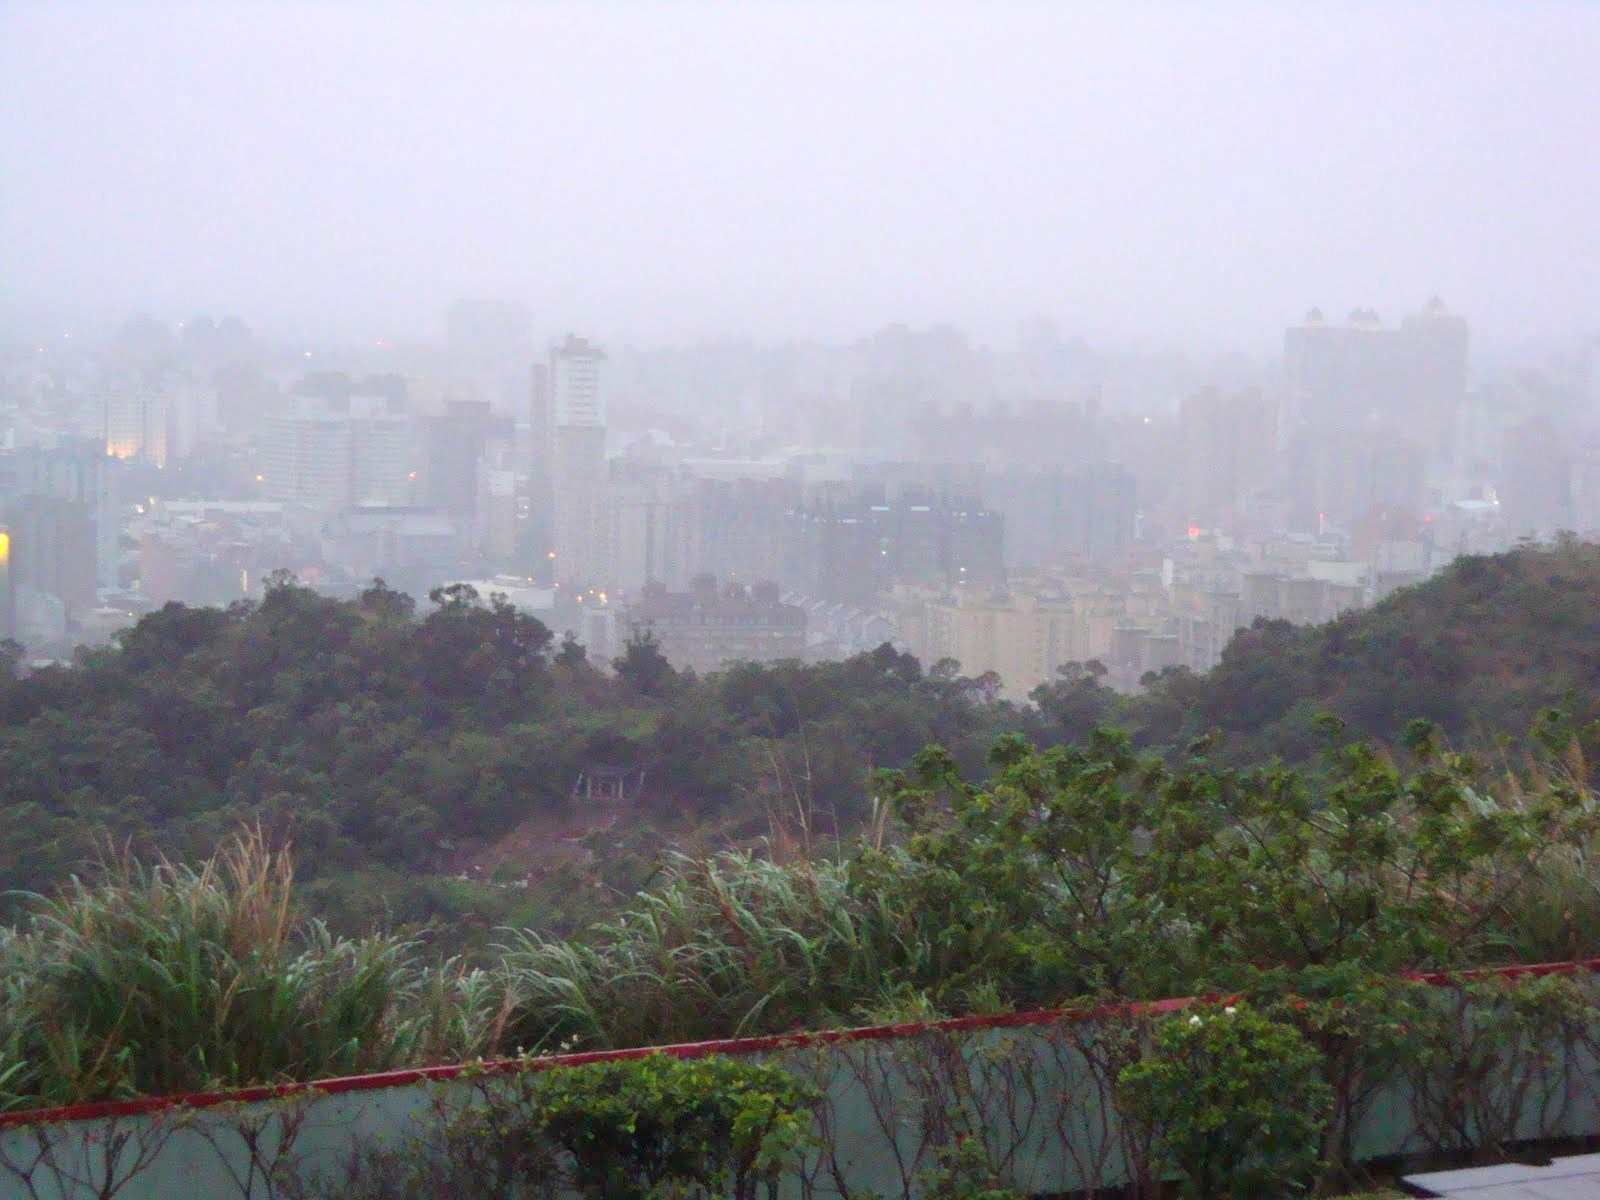
\includegraphics[height=2in]{notes/media/air_pollution.jpg}
  \end{center}
\end{frame}

\begin{frame}
  \frametitle{Набір даних}

  Загальний опис датасету:

  \begin{enumerate}
    \item Кількість рядків: 5\,882\,208
    \item Кількість стовпців: 25

    \begin{itemize}
      \item Числові: 19
      \item Факторні: 4
      \item Дата: 1
      \item Інші: 1
    \end{itemize}
  \end{enumerate}
\end{frame}

\begin{frame}
  \frametitle{Питання EDA}

  \begin{enumerate}
    \item Чи впливає швидкість вітру на концентрацію частинок PM2.5 і PM10?
    \item Чи існує кореляція між рівнем забруднення повітря і типом головного забруднювача
    в різних районах?
    \item Як зміни в концентрації озону  впливають на загальний рівень забруднення повітря?
    \item Які регіони мають найвищий середній рівень забруднення повітря протягом року?
    \item Як змінюється якість повітря протягом доби в різних районах?
  \end{enumerate}
\end{frame}

\begin{frame}
  \frametitle{Питання EDA}

  \begin{enumerate}
    \setcounter{enumi}{5}

    \item Як змінюється концентрація PM2.5 і PM10 в залежності від швидкості вітру і напрямку вітру
    в різних регіонах?
    \item Як змінився загальний рівень забруднення по регіонам після початку реформи?
    \item Чи існує залежність між початком реформ та показниками забруднення?
    \item Як змінюється якість повітря залежно від станції виміру у містах?
  \end{enumerate}
\end{frame}

\begin{frame}
  \section{Підготовка даних}

  \frametitle{Зміст}
  \tableofcontents[currentsection]
\end{frame}

\begin{frame}
  \frametitle{"Очищення" даних}

  \begin{enumerate}
    \item Перетворили кодові значення на NA.
    \item Видалили стовбці, які не знадобляться для аналізу.
    \item Видалили стовбці, в яких більше $50\%$ пропущених даних.
    \item Додали стовбець \textit{after\_reform}, що визначає, чи вимір
    якості повітря був здійнений після реформи (\textit{17 грудня 2017 року})
  \end{enumerate}
\end{frame}

\begin{frame}
  \frametitle{"Очищення" даних}

  Був отриманий набір даних, що складається з таких змінних:

  \begin{itemize}
    \item Факторні - 3
    \item Логічні - 1
    \item Числові - 11
    \item Дата - 1
  \end{itemize}
\end{frame}

\begin{frame}
  \frametitle{Зменшення датасету}

  \begin{enumerate}
    \item Для пришвидшення обчислень та побудови графіків в певних випадках будемо використовувати
    окремий набір даних, в якому виміри починаються з 2023 року.
    \item Таким чином цей набір даних має 1\,232\,994 рядків.
    \item Надалі будемо зазначати на якому наборі даних був виконаний аналіз. Зменшений
    датасет назвемо \textit{trimmed}, весь очищений набір даних -- \textit{tidy}.
  \end{enumerate}

\end{frame}

\begin{frame}
  \section{Характеристика даних}

  \frametitle{Зміст}
  \tableofcontents[currentsection]
\end{frame}

\begin{frame}
  \frametitle{Пропущені дані}

  Був використаний \textit{tidy} набір даних.

  \begin{center}
    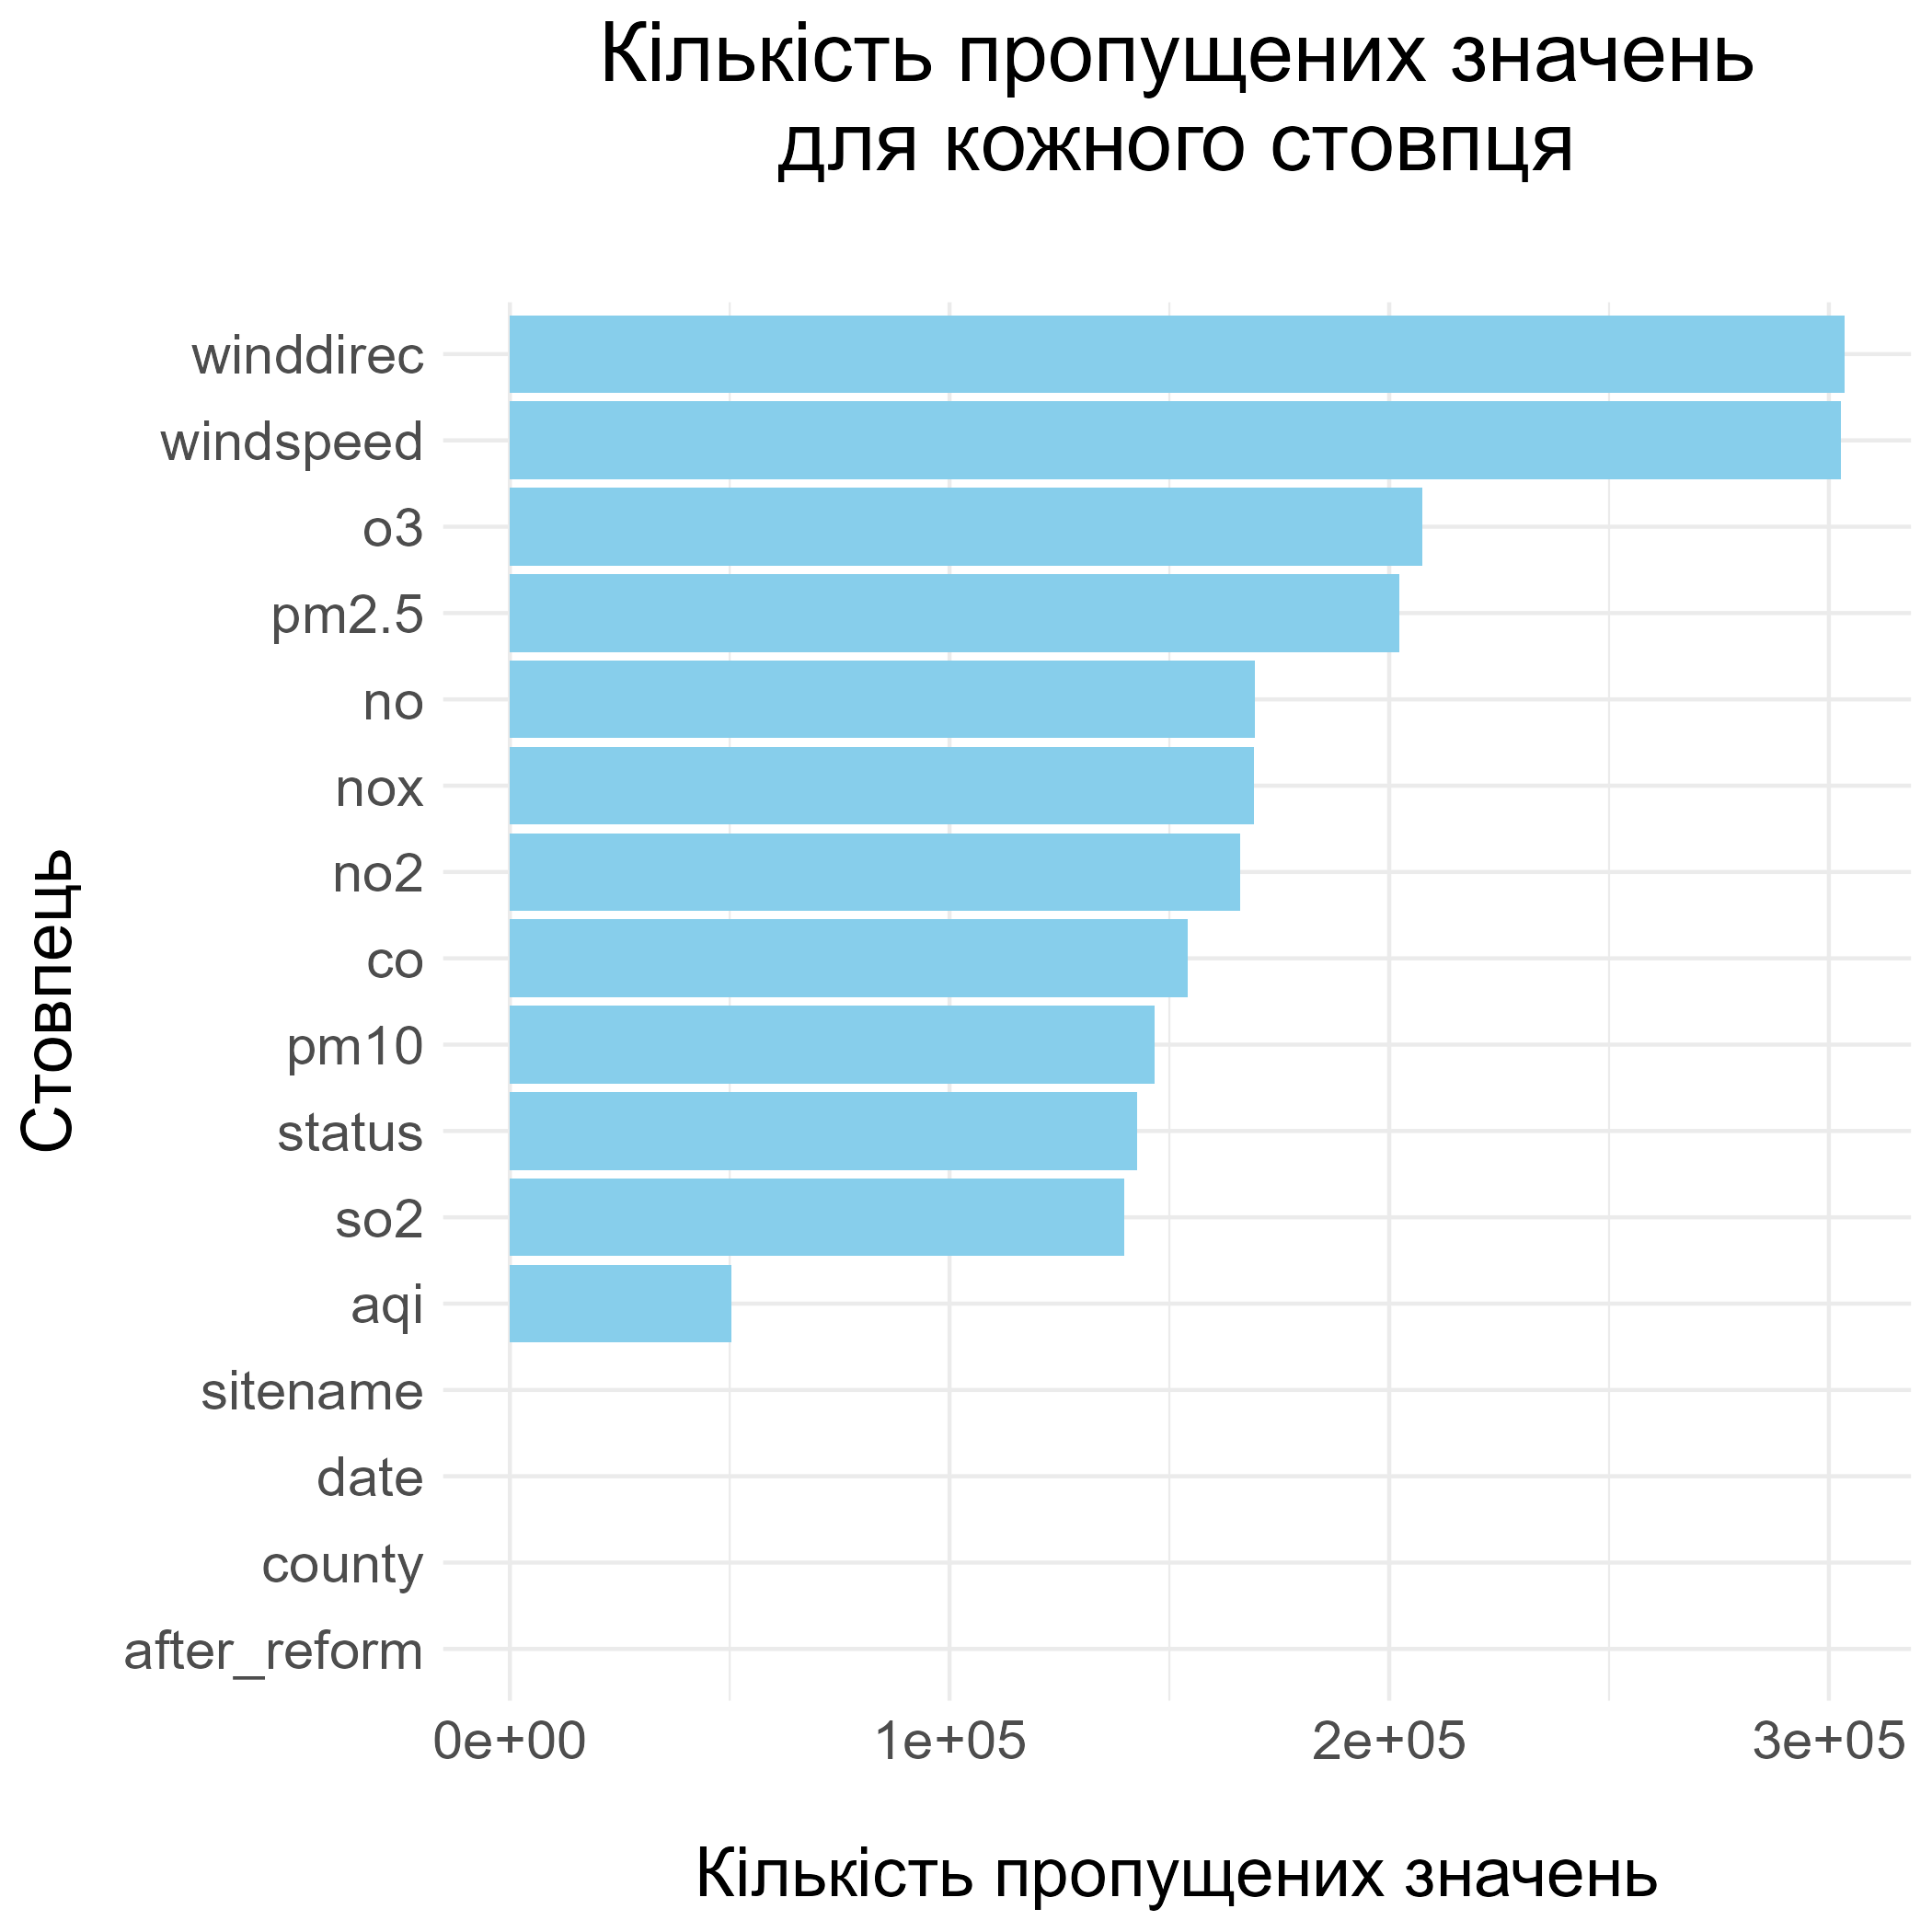
\includegraphics[height=2.8in]{plots/missed_data.png}
  \end{center}
\end{frame}

\begin{frame}
  \frametitle{Викиди}

  Був використаний \textit{trimmed} набір даних.

  Для пошуку викидів використаємо \textit{фільтр Гампеля}:

  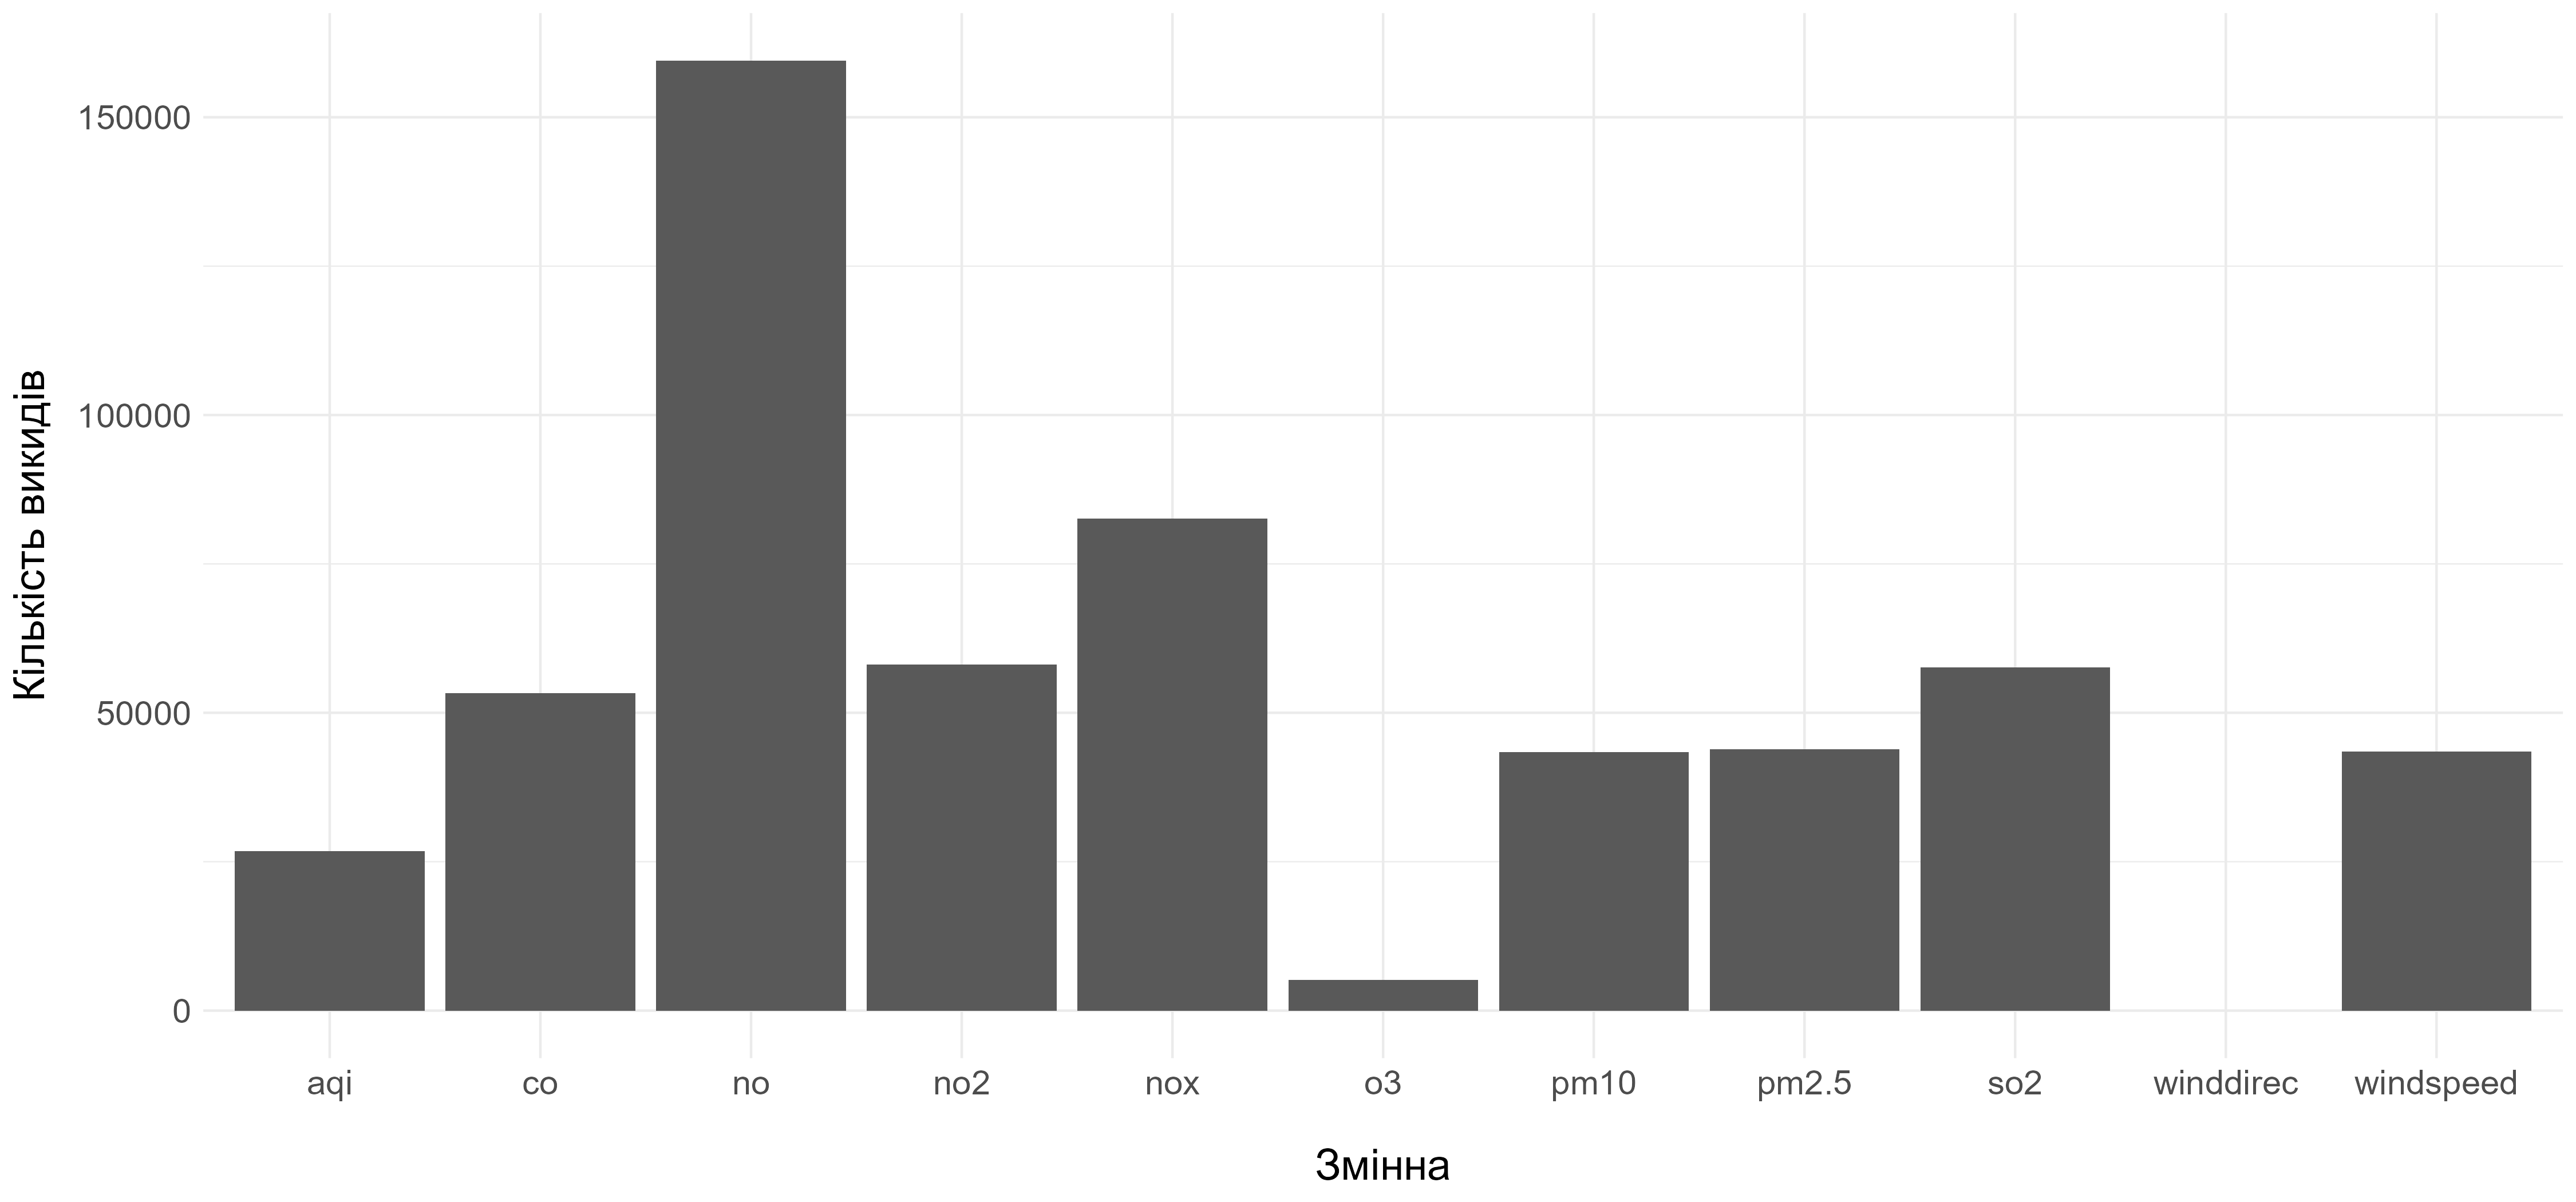
\includegraphics[width=\linewidth]{plots/outliers/count-bar.png}
\end{frame}

\begin{frame}
  \frametitle{Викиди}

  \begin{center}
    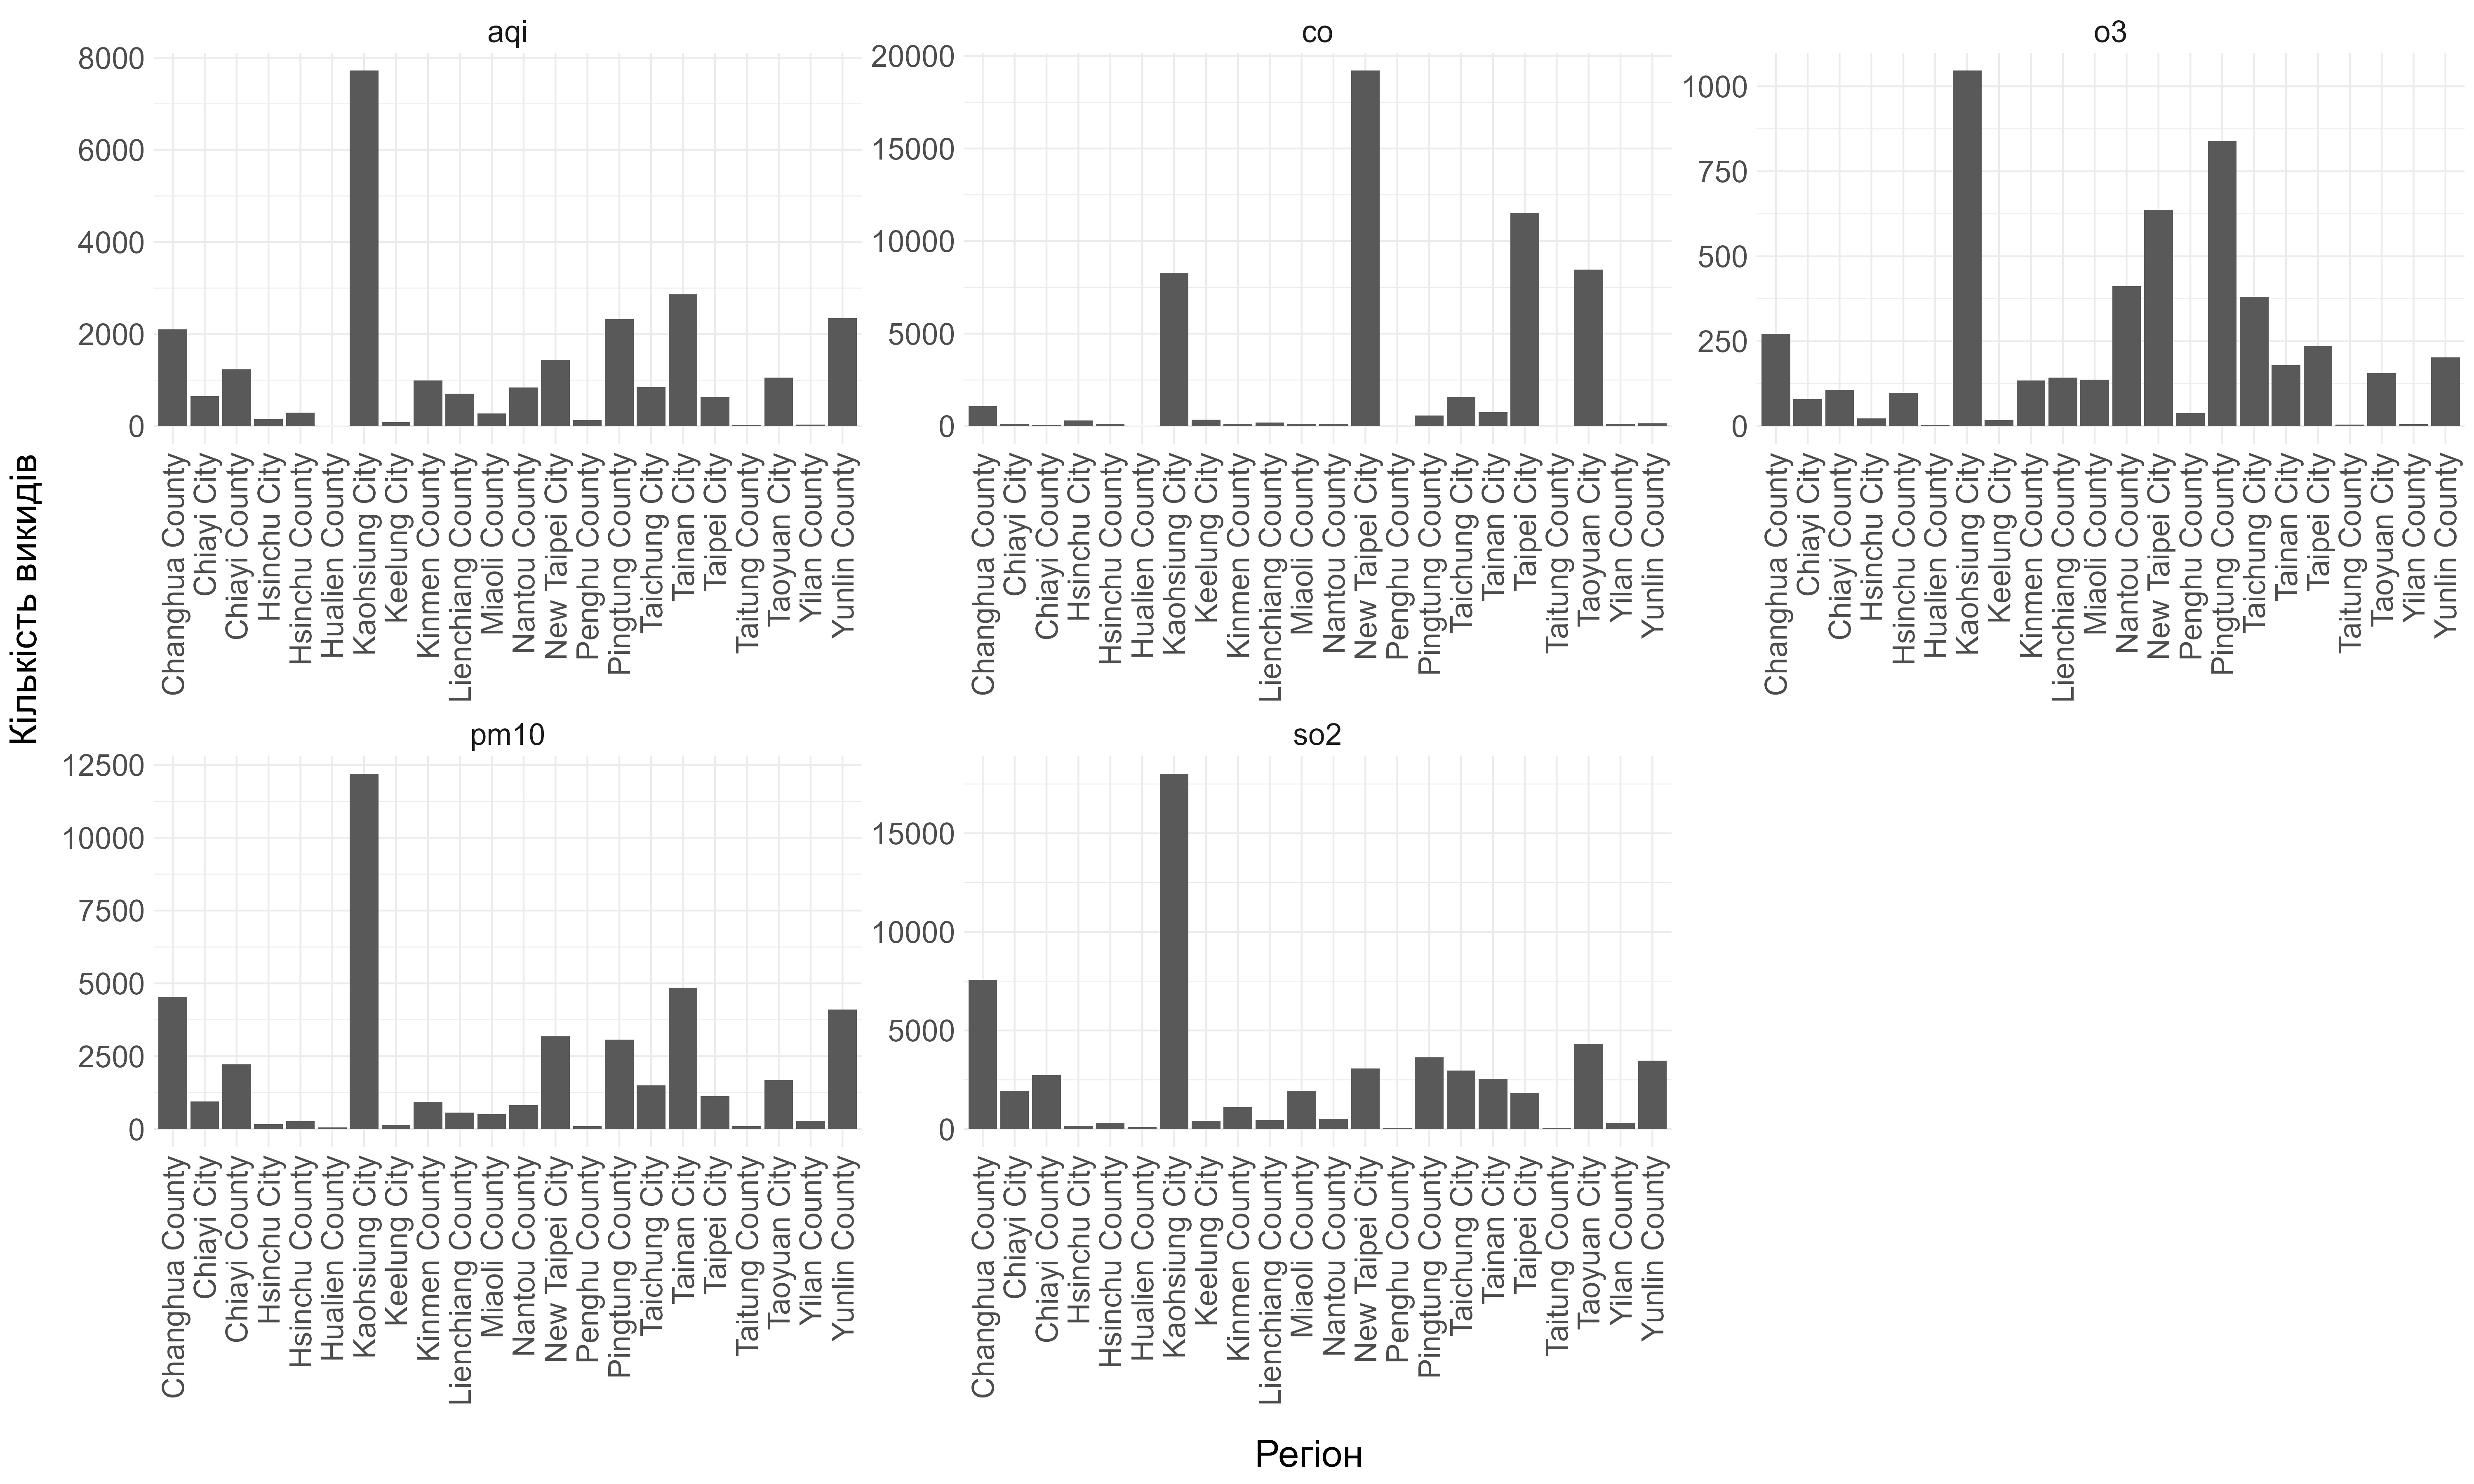
\includegraphics[height=3in]{plots/outliers/count-bar-county-p1.png}
  \end{center}
\end{frame}

\begin{frame}
  \frametitle{Викиди}

  \begin{center}
    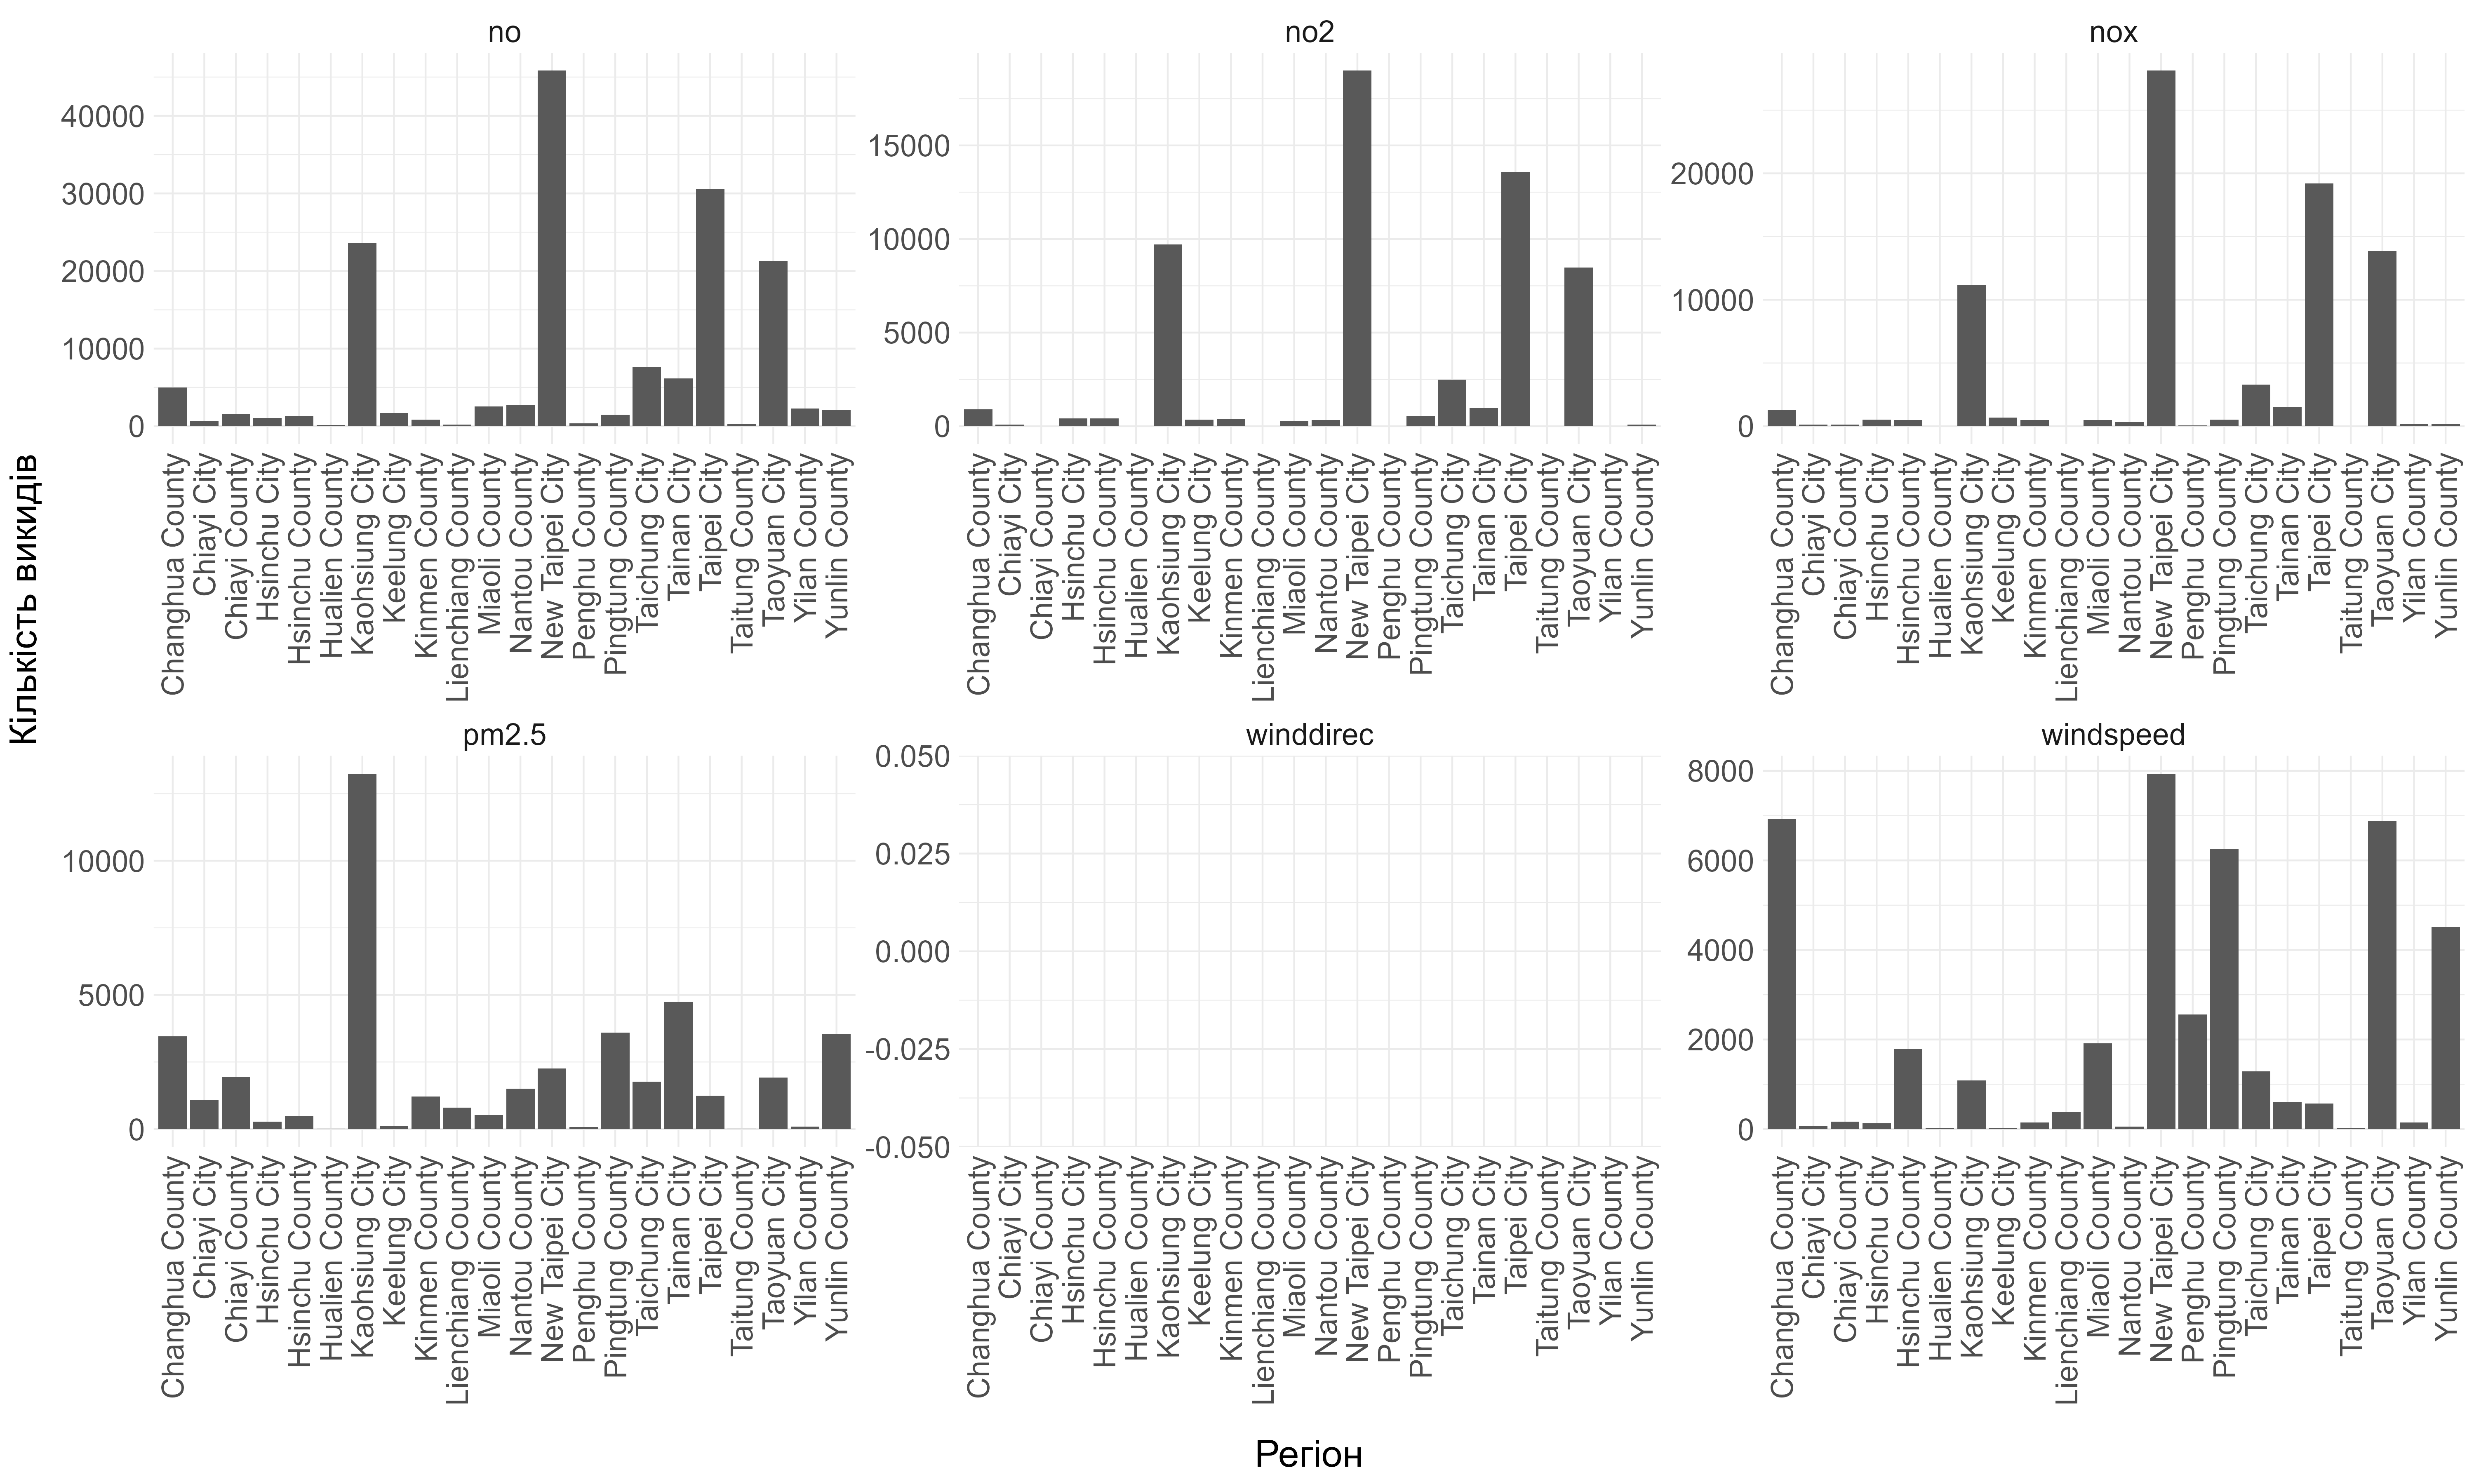
\includegraphics[height=3in]{plots/outliers/count-bar-county-p2.png}
  \end{center}
\end{frame}

\begin{frame}
  \frametitle{Викиди}

  \begin{center}
    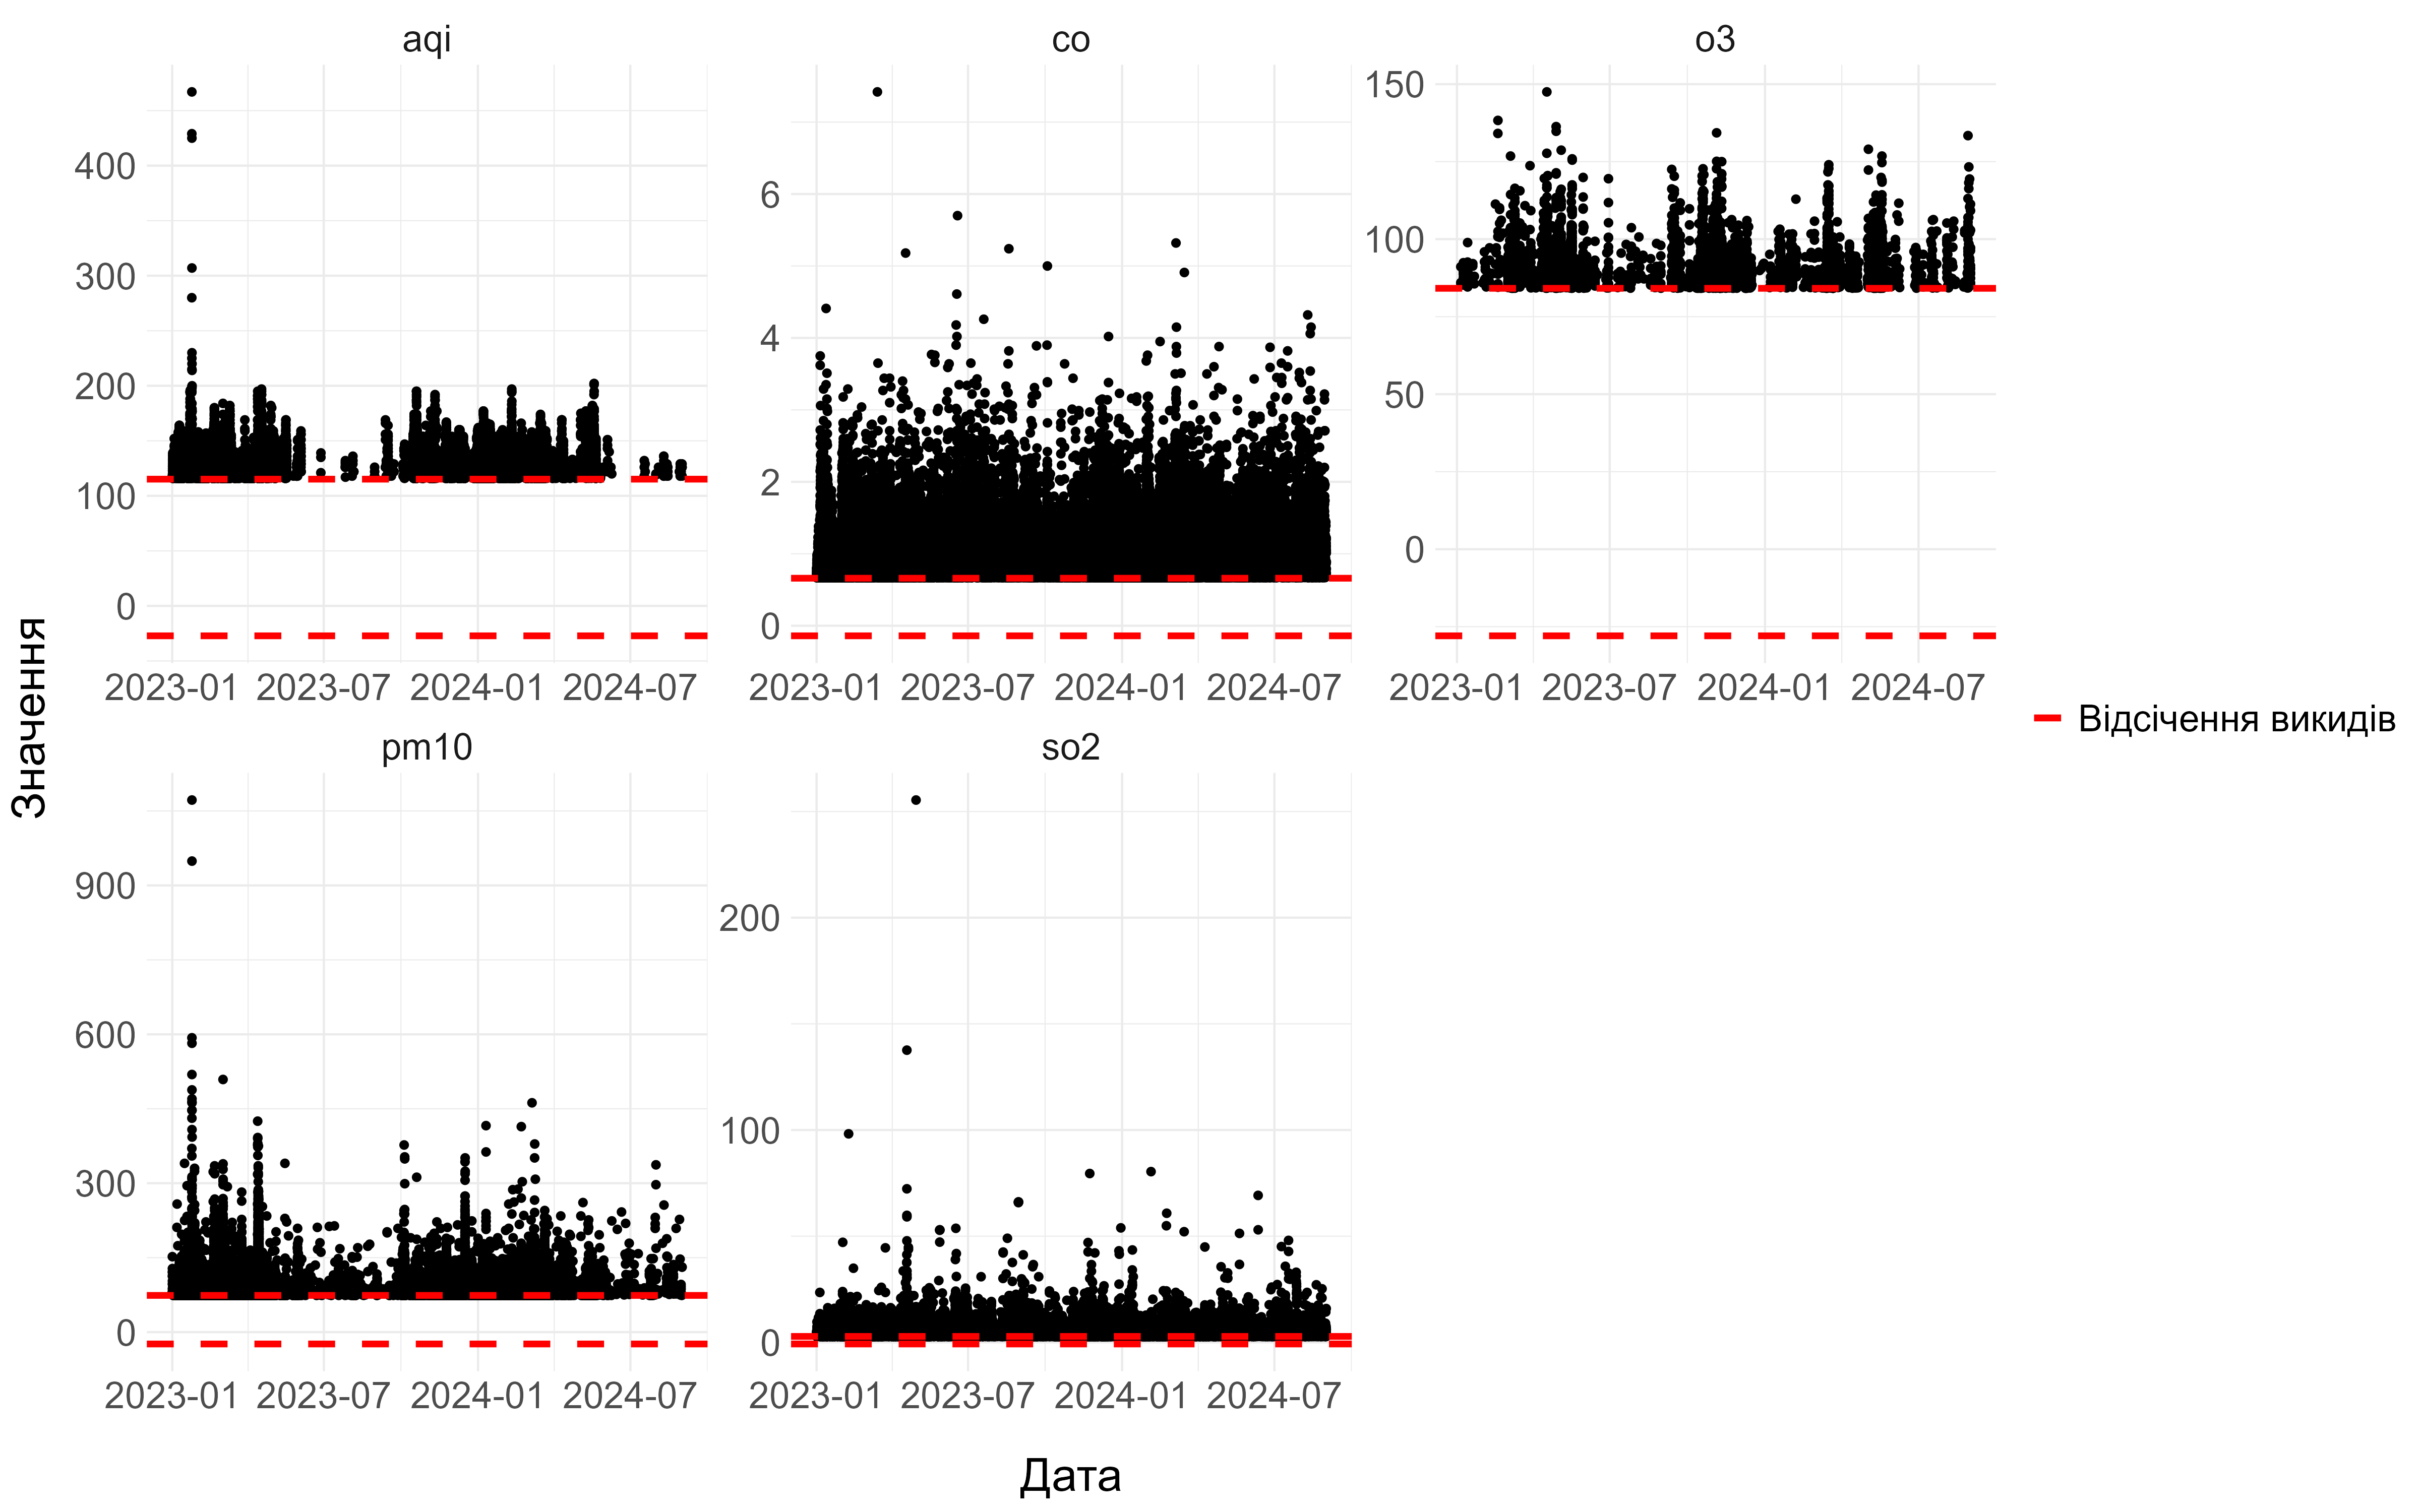
\includegraphics[height=3in]{plots/outliers/scatter-p1.png}
  \end{center}
\end{frame}

\begin{frame}
  \frametitle{Викиди}

  \begin{center}
    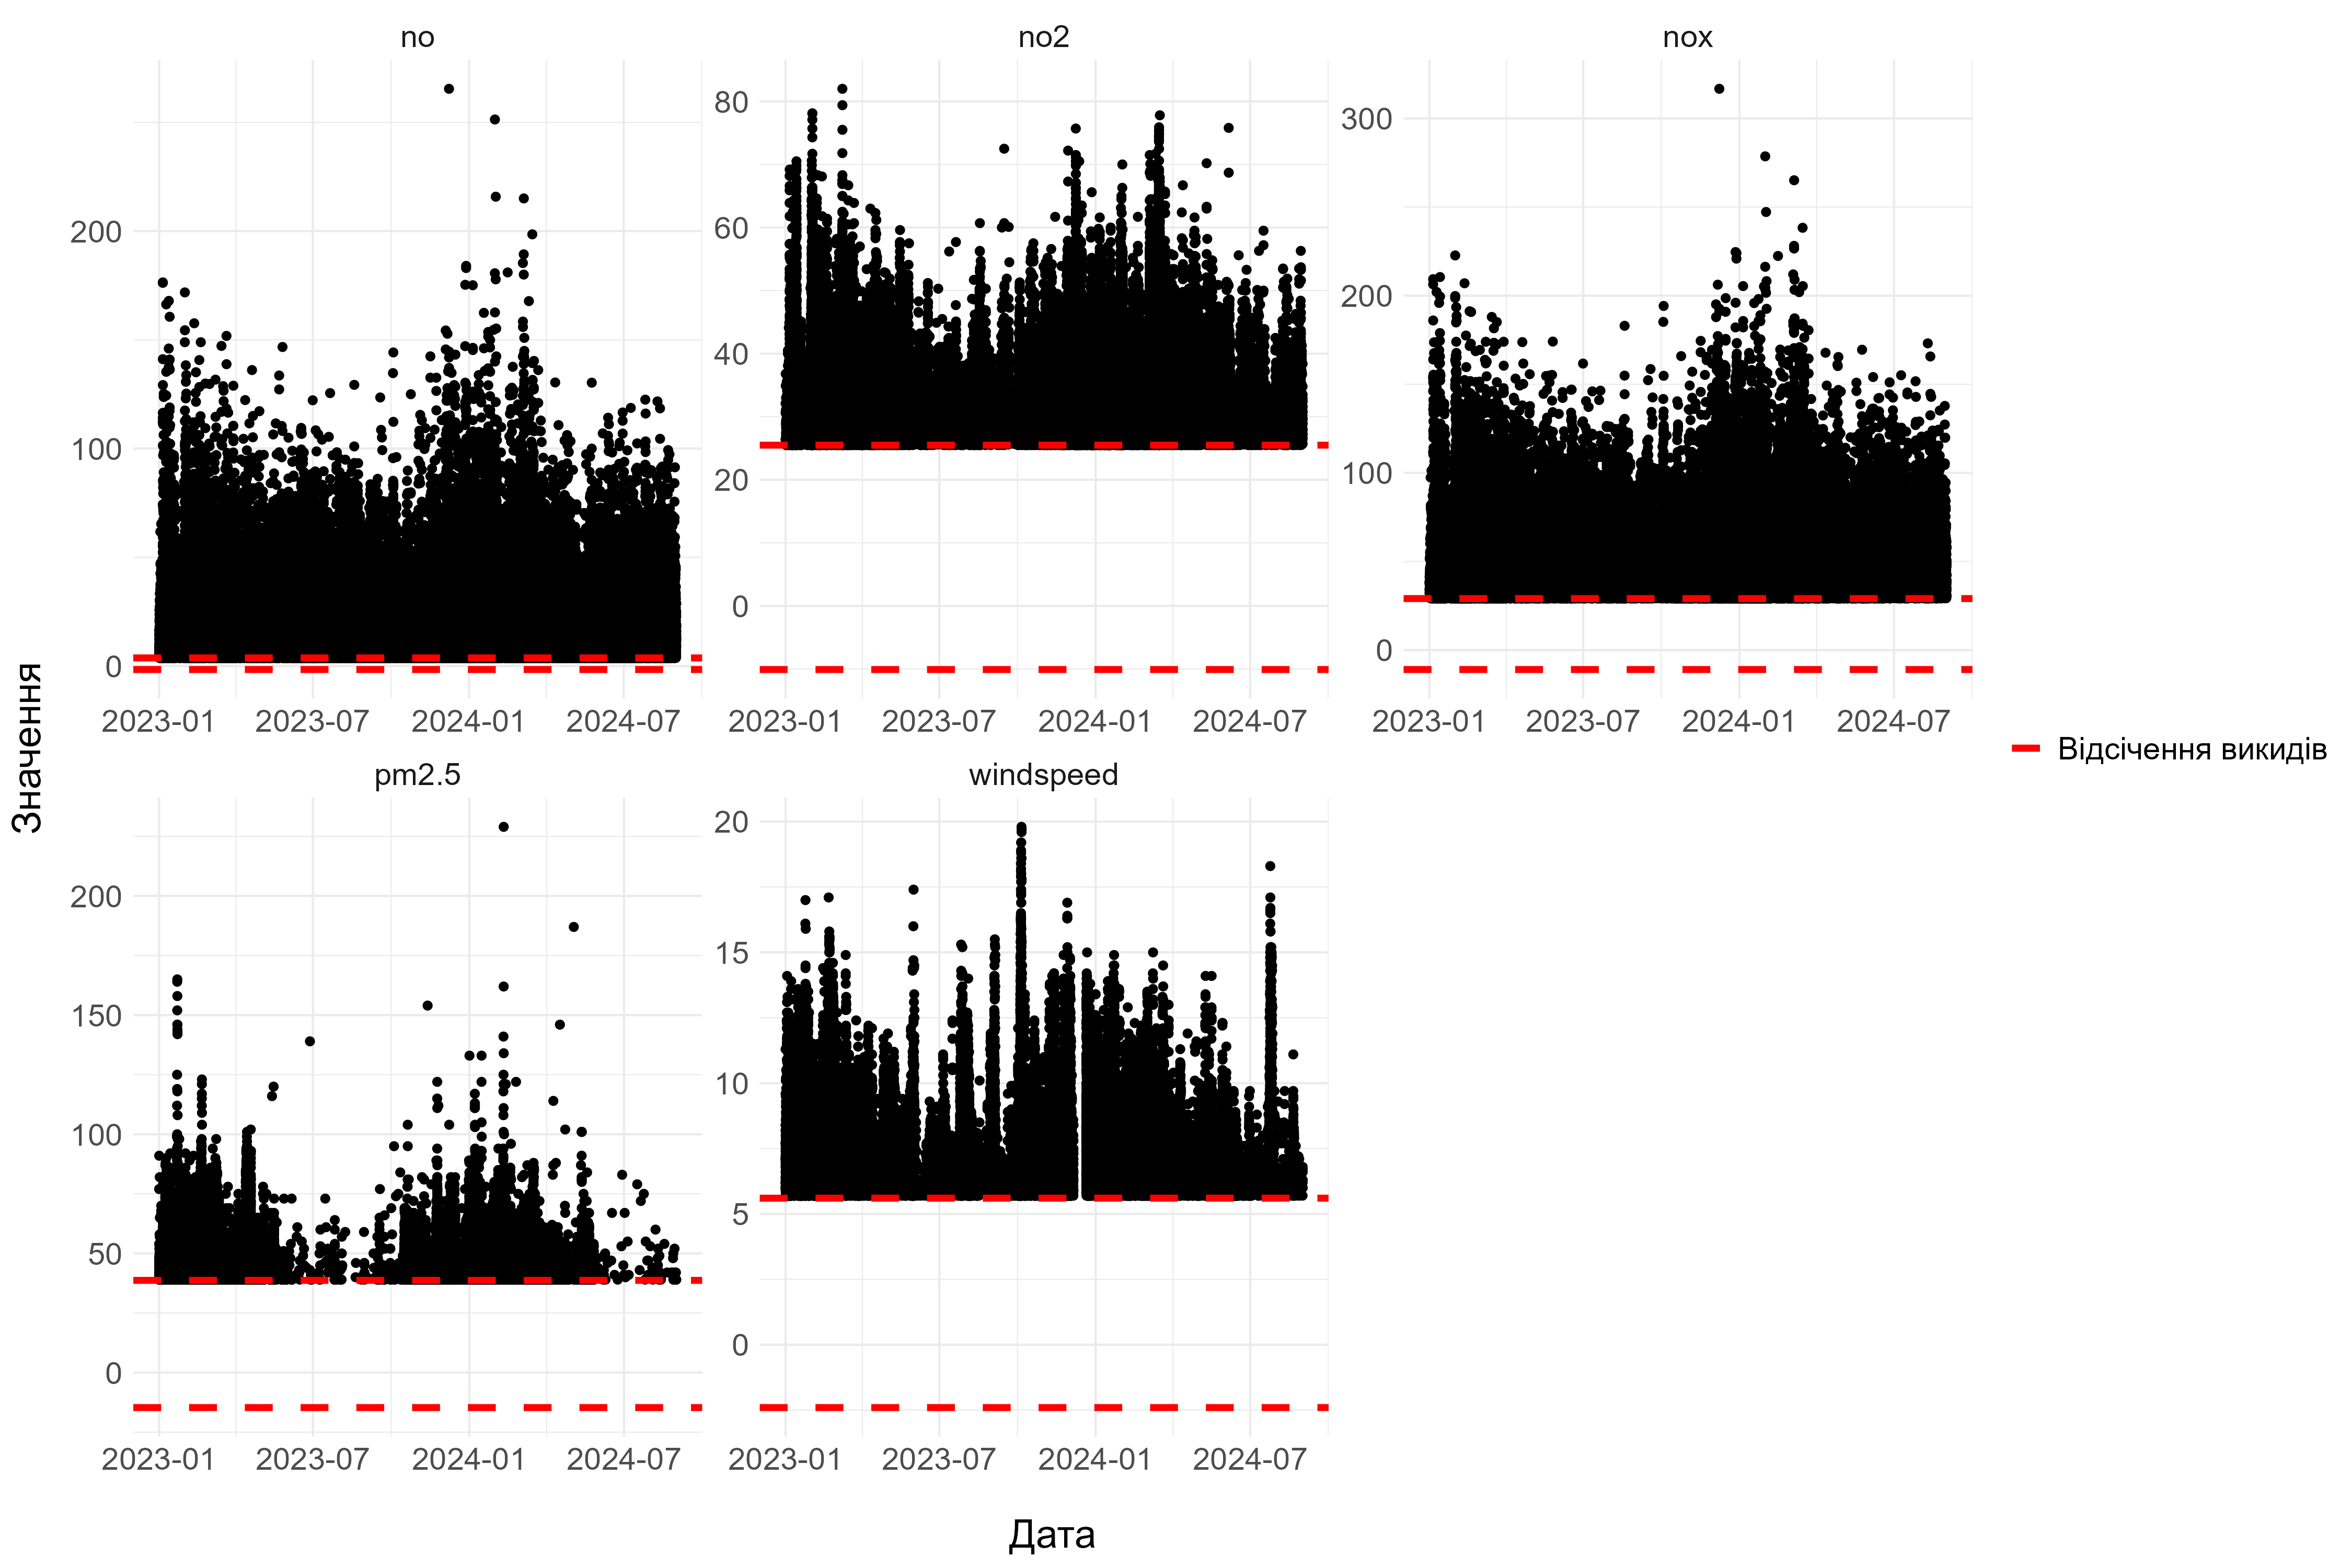
\includegraphics[height=3in]{plots/outliers/scatter-p2.png}
  \end{center}
\end{frame}

\begin{frame}
  \frametitle{Викиди}

  \begin{enumerate}
    \item На діаграмі розсіювання можна замітити значення, які набагато більші за
    інші викиди. Можна припустити, що вони є помилками датників, які вимірювали якість
    повітря.
    \item  Було прийнято рішення не змінювати значення, або видаляти викиди.
    Натомість будемо використовувати міри, які більш стійкі до викидів.
  \end{enumerate}
\end{frame}

\begin{frame}
  \frametitle{Розподіли змінних}

  Для побудови QQ-графіків, випадковим чином виберемо з датасету 10\,000 рядків.

  \begin{center}
    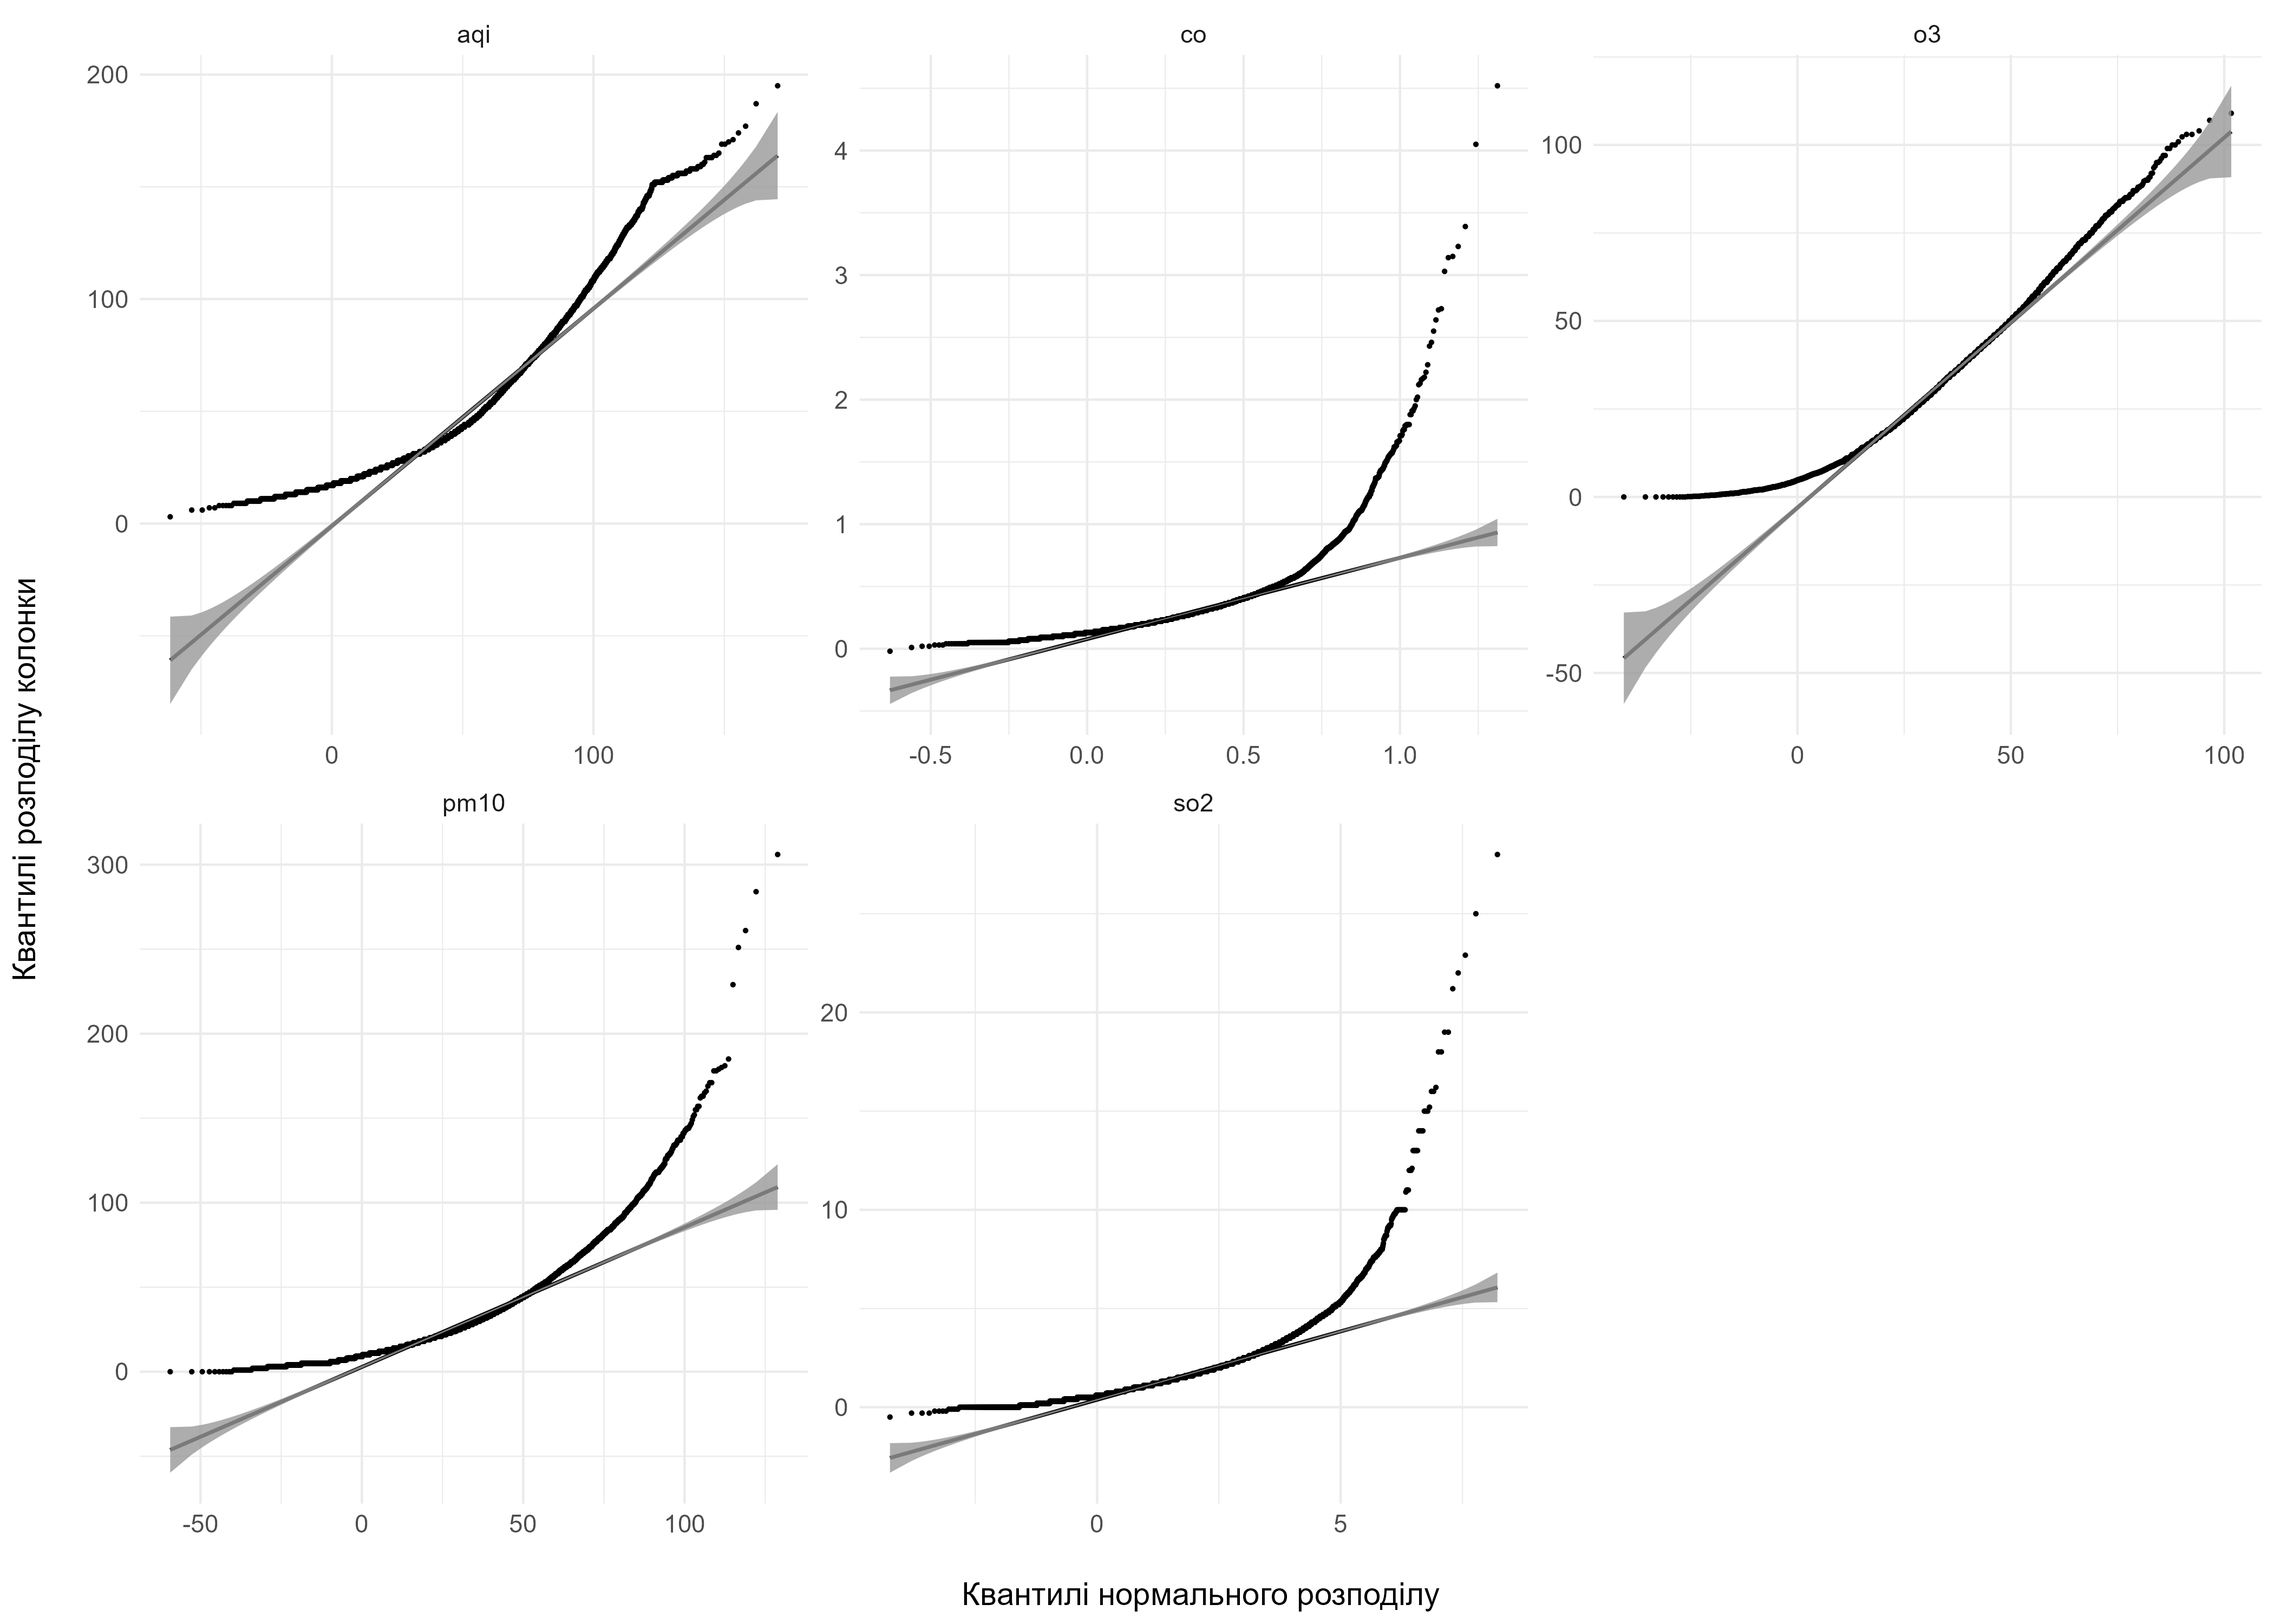
\includegraphics[height=2.5in]{plots/qq_tidy/qq-p1.png}
  \end{center}
\end{frame}

\begin{frame}
  \frametitle{Розподіли змінних}

  \begin{center}
    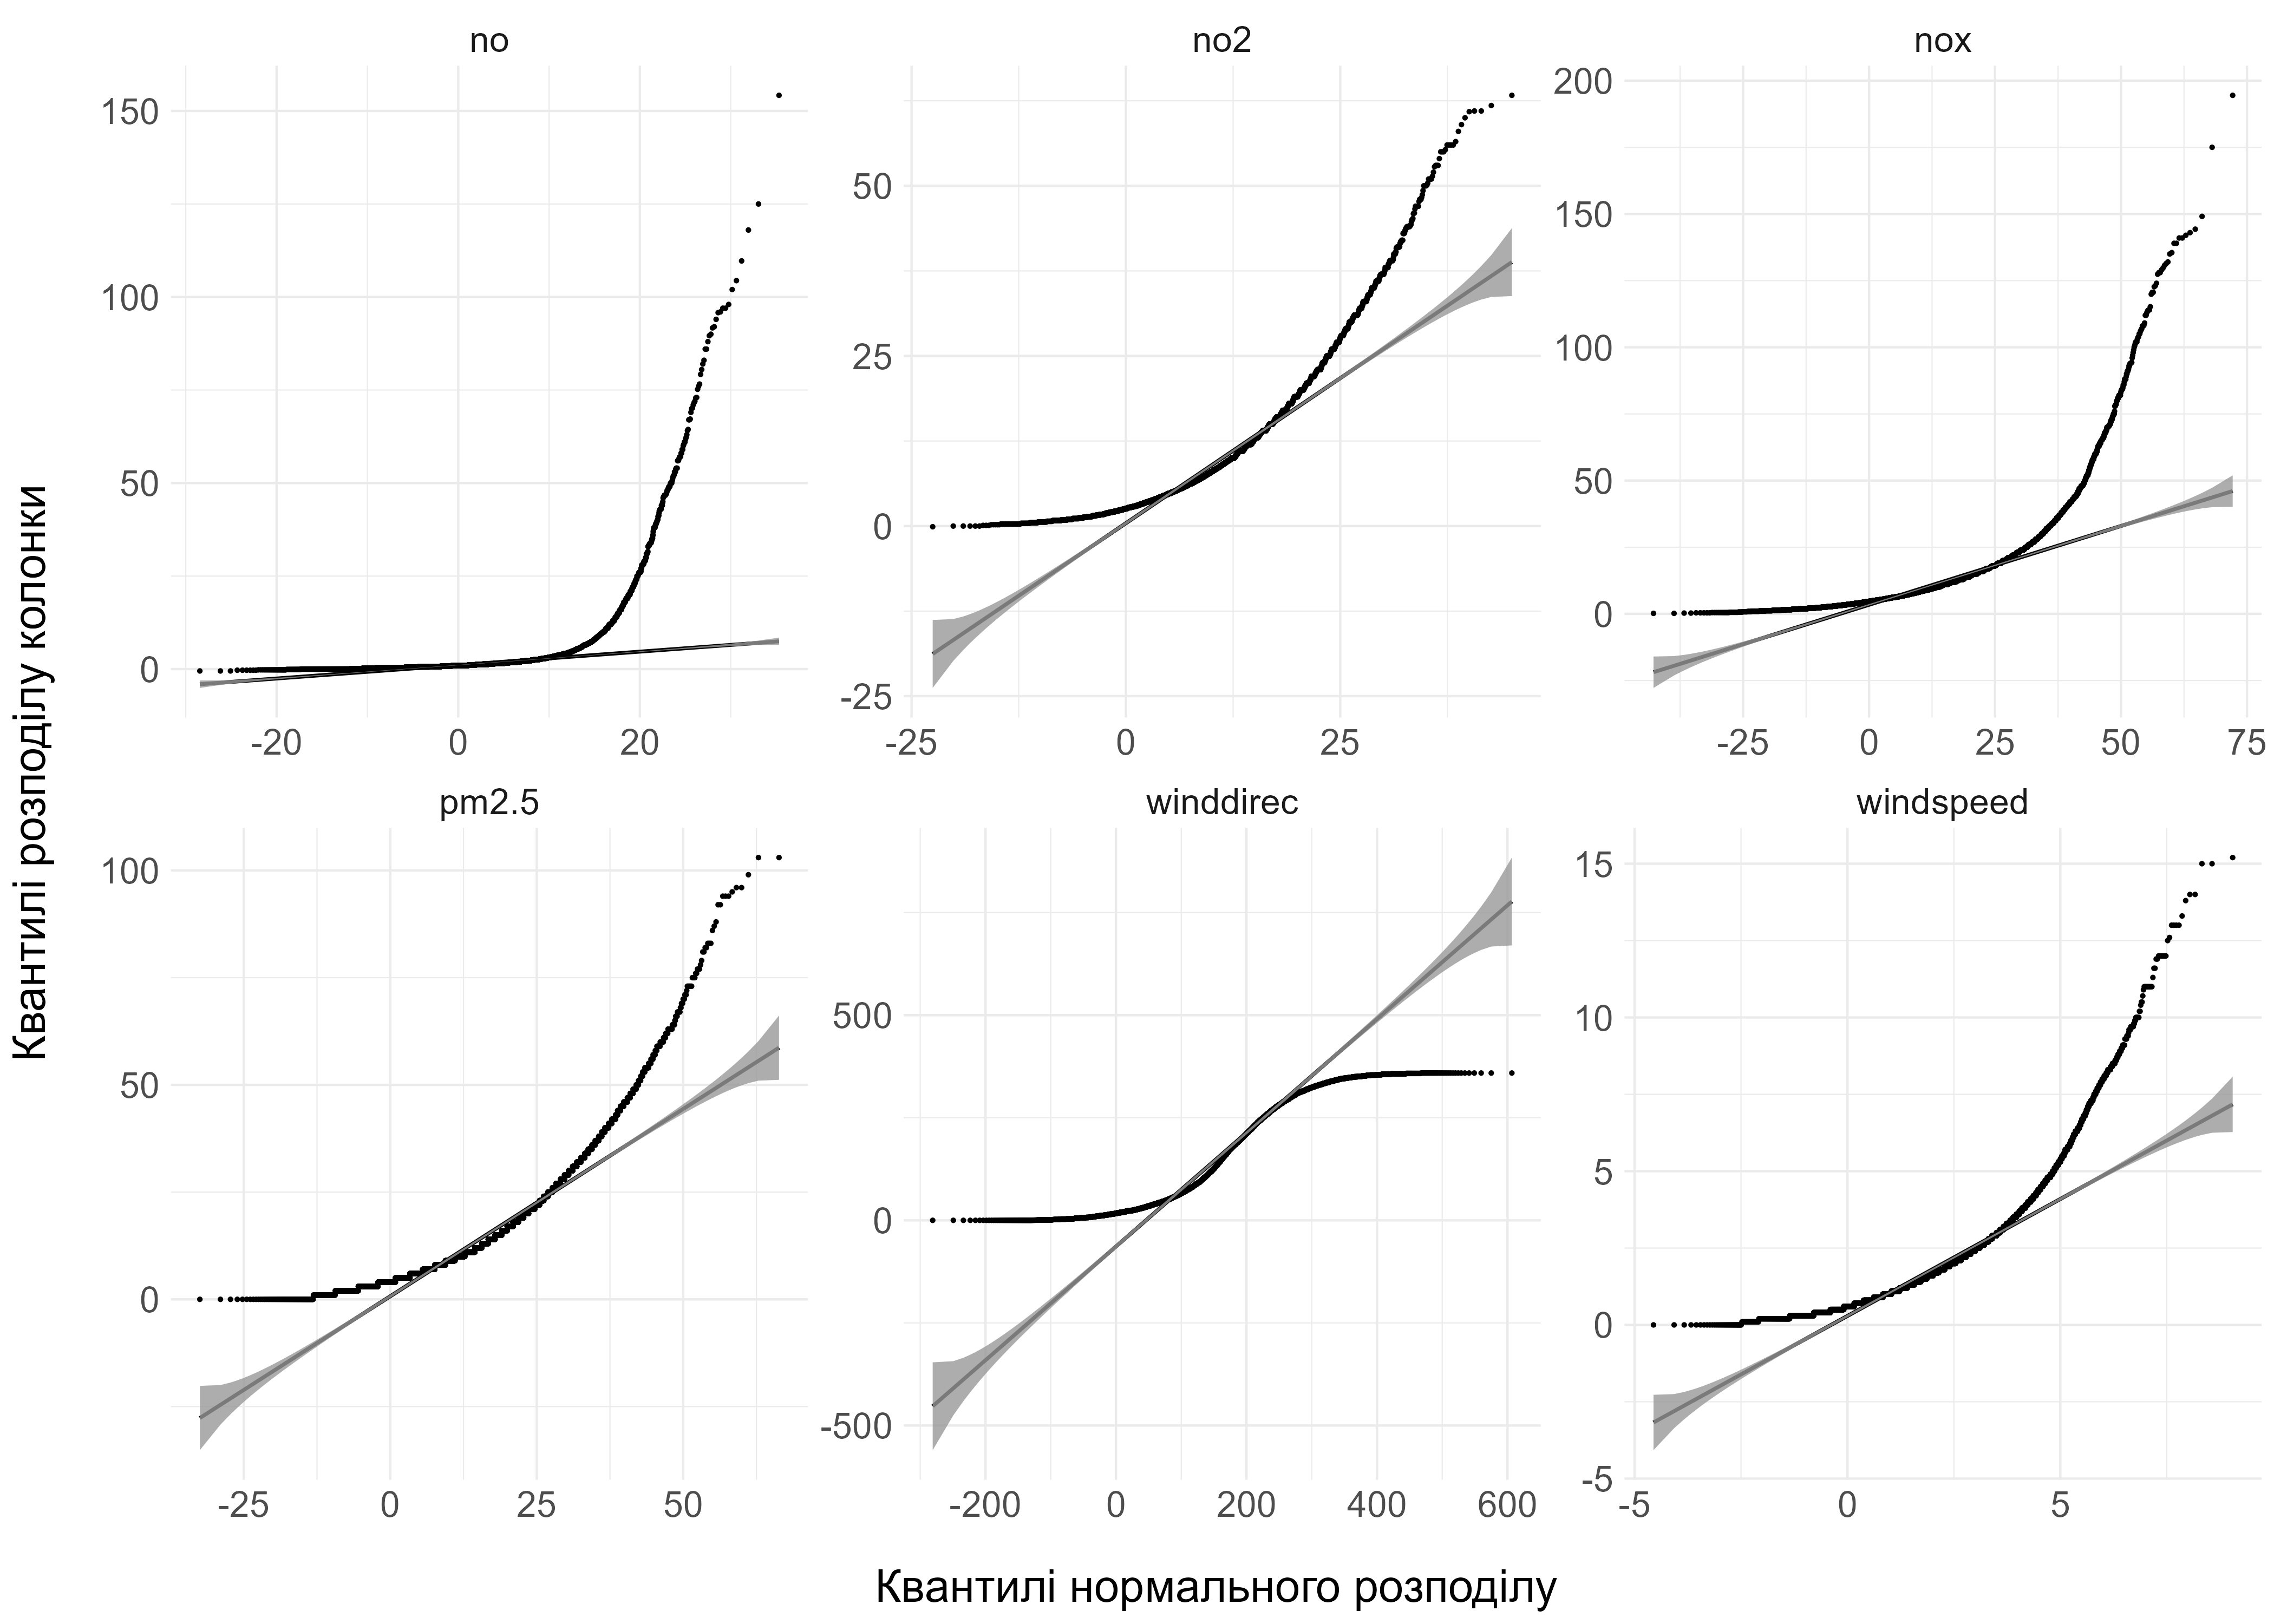
\includegraphics[height=3in]{plots/qq_tidy/qq-p2.png}
  \end{center}
\end{frame}

\begin{frame}
  \frametitle{Розподіли змінних}

  Розподіл змінних (крім \textit{winddirect}) ближче до логнормального, ніж нормального:

  \begin{center}
    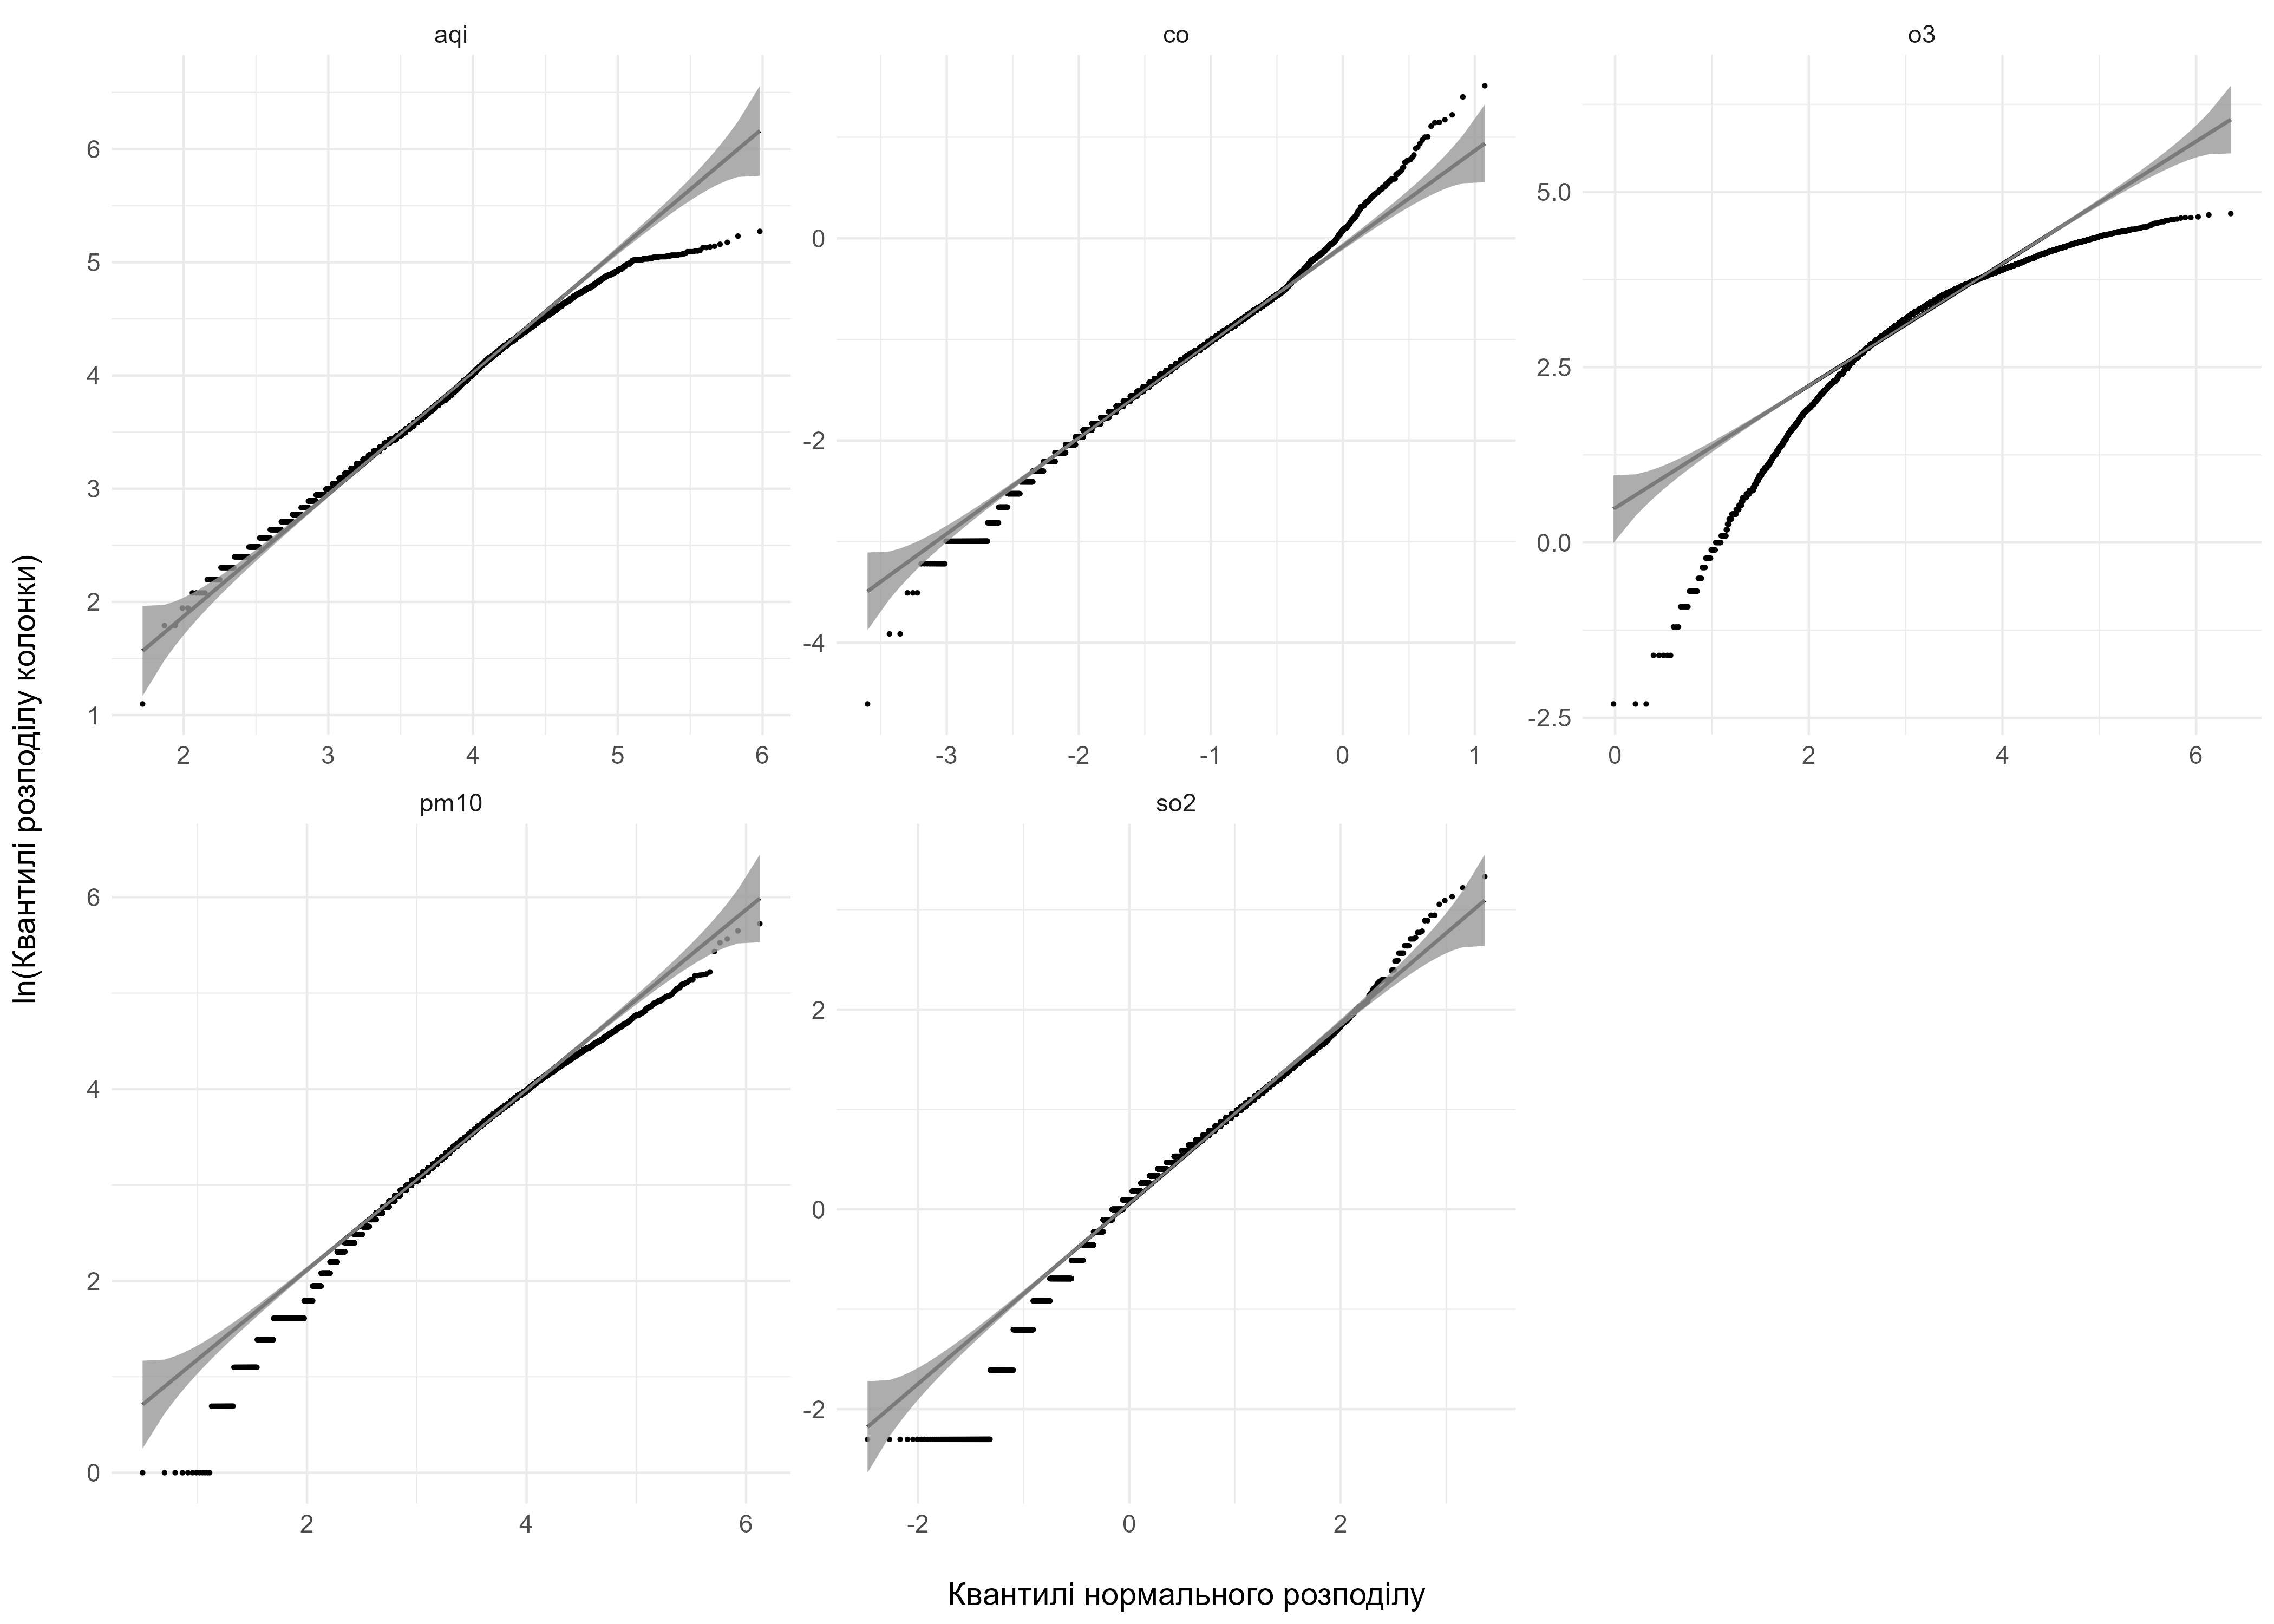
\includegraphics[height=2.5in]{plots/qq_tidy/qq-log-p1.png}
  \end{center}
\end{frame}

\begin{frame}
  \frametitle{Розподіли змінних}

  \begin{center}
    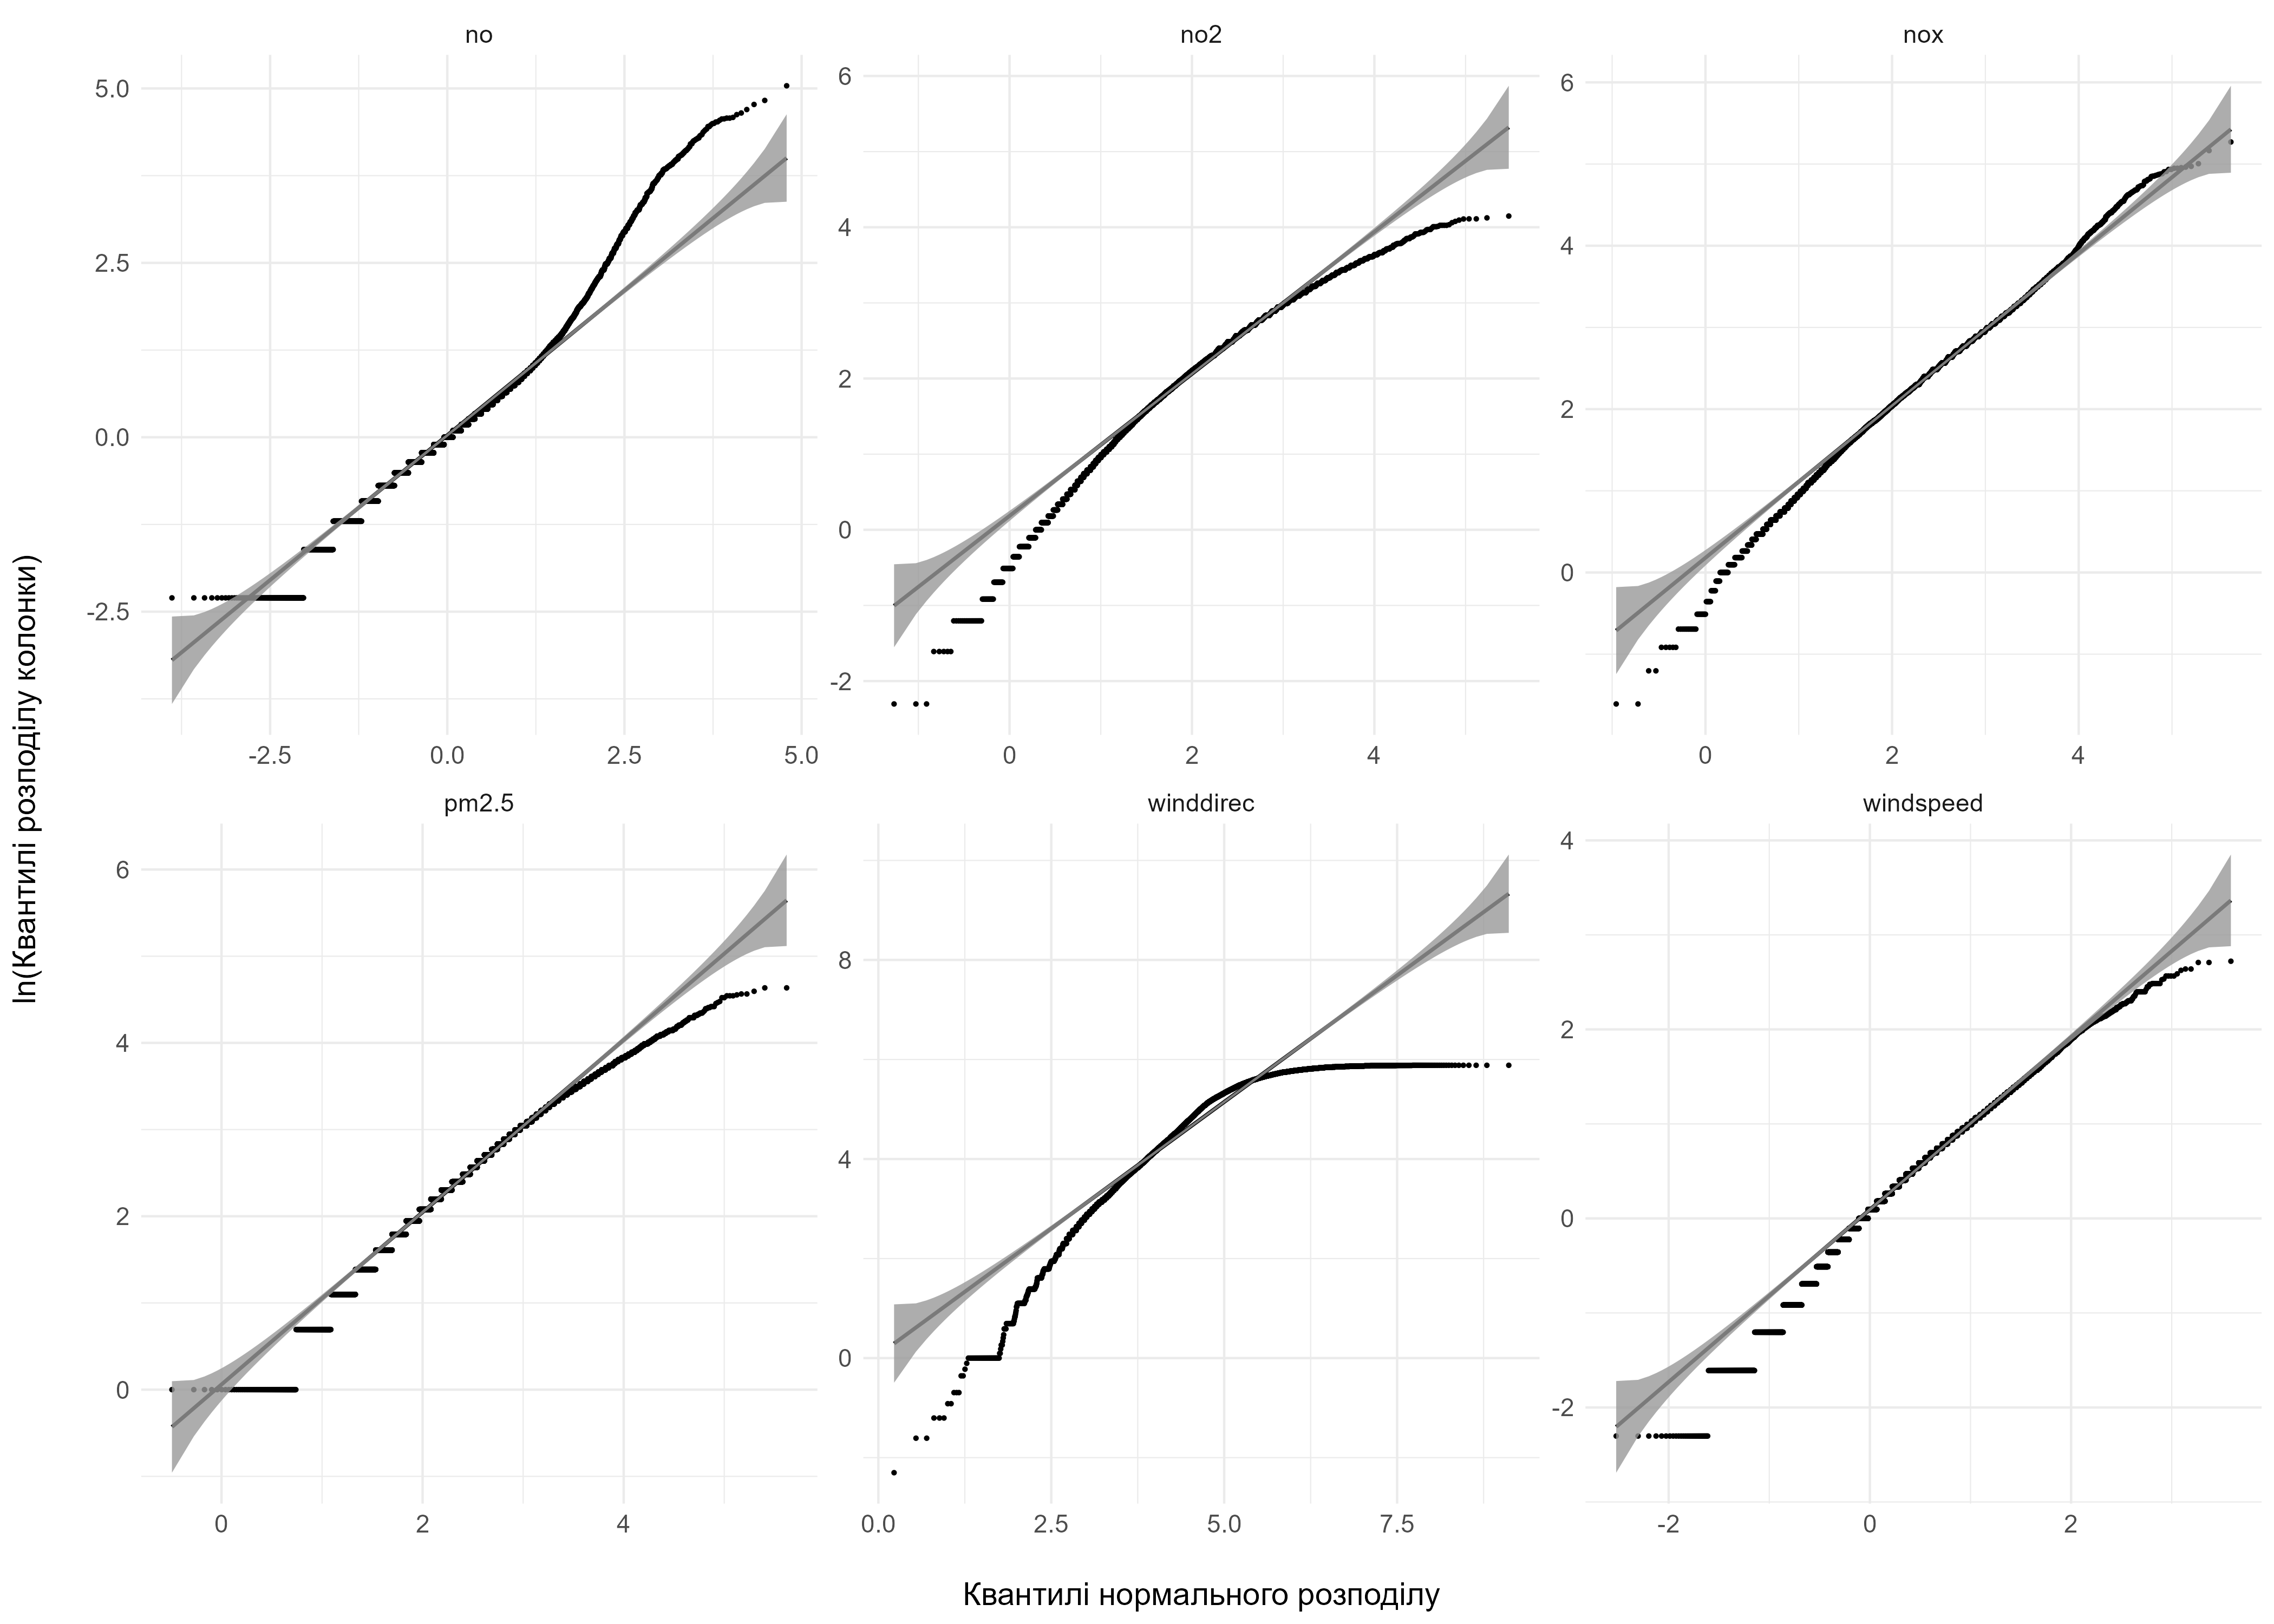
\includegraphics[height=3in]{plots/qq_tidy/qq-log-p2.png}
  \end{center}
\end{frame}


\begin{frame}
  \section{Питання EDA}

  \frametitle{Зміст}
  \tableofcontents[currentsection]
\end{frame}

\end{document}